\documentclass[a4paper,12pt]{report}
\usepackage[a4paper, total={7in, 10in}]{geometry}
\usepackage{graphicx} % For including images
\usepackage{amsmath}  % For mathematical symbols
\usepackage{tocbibind}
\setcounter{secnumdepth}{4}
\usepackage[justification=centering]{caption}
\usepackage{enumitem}
\usepackage{makecell}
\usepackage[table]{xcolor} % Required for table coloring
\usepackage{array}
\usepackage{float} % ضيفه في preamble
\usepackage{colortbl}
\usepackage[colorlinks=true, linkcolor=black, urlcolor=black, citecolor=black]{hyperref}
\usepackage[noprefix]{nomencl} % Package to create a list of acronyms
\usepackage[linesnumbered,ruled,vlined]{algorithm2e}
\usepackage{listings}
\usepackage{tcolorbox}
\tcbuselibrary{listingsutf8}
\usepackage[backend=biber,style=ieee]{biblatex}
\renewcommand*{\revsdnamepunct}{}  % لمنع الشرطة الطويلة عند نفس المؤلف
\addbibresource{references.bib}
\usepackage{pdfpages}  % في preamble
\usepackage{tikz}
\usepackage{hyperref}





\makenomenclature % Create the nomenclature (list of acronyms)

\begin{document}


\begin{titlepage}
    \centering
    
\includegraphics[width=0.6\textwidth]{figure/PPU.png}\\[0.3cm]
    {\Huge\textbf{Palestine Polytechnic University}}\\[0.7cm]
    {\large\textbf{College of Information Technology and Computer Systems Engineering}}\\[0.2cm]
    {\large\textbf{Department of Computer Systems Engineering}}\\[1.5cm] 
    {\Huge \textbf{AutiSense: \\[0.1cm]Smart Assistant System for Children with Autism Spectrum Disorder }}\\[2cm]
    {\large\textbf{Authors:}}\\[0.3cm]
    {\large\textbf{Batool Shaheen - 237010}}\\[0.3cm]
    {\large\textbf{Raghad Darabee - 237008}}\\[2cm]
    {\large\textbf {Supervised by:}}\\[0.3cm]
    {\large\textbf {Eng. Wael Altakrouri}}\\[2cm]
    {\large\textit{To fulfill the requirements for a bachelor’s degree in Computer Systems Engineering}}\\[1.5cm]
    \textbf{2025-2026}
    \vfill
\end{titlepage}



% Table of Contents
\tableofcontents
\clearpage

% List of Figures
\listoffigures
\clearpage

% List of Tables
\listoftables
\clearpage

\setlength{\nomlabelwidth}{3cm} % عرض عمود الاختصارات
\renewcommand{\nomlabel}[1]{#1 \hfill}

% List of Acronyms
\renewcommand{\nomname}{List of Acronyms} % تغيير العنوان
\nomenclature{ASD}{ Autism Spectrum Disorder}
\nomenclature{IDEA}{ Individuals with Disabilities Education Act}
\nomenclature{DSM}{Diagnostic and Statistical Manual of Mental Disorders}
\nomenclature{EBD}{ Emotional Behavior Disorder}
\nomenclature{IDE}{ Integrated Development Environment}
\nomenclature{EDA}{Electrodermal activity}
\nomenclature{HRV}{Heart Rate Variability}
\nomenclature{PPG}{Photoplethysmography}
\nomenclature{BPM}{heartbeats per minute}
\nomenclature{GSR}{Galvanic Skin Response}
\nomenclature{HR}{Heart Rate}
\nomenclature{MPU}{Motion Processing Unit}
\nomenclature{ADXL335}{Analog Devices Acceleromete}
\nomenclature{DMP}{Digital Motion Processor}
\nomenclature{SVM}{Support Vector Machine}
\nomenclature{PWM}{Pulse Width Modulation}
\nomenclature{GPU}{Graphics Processing Unit }
\nomenclature{LCD}{Liquid Crystal Display}
\nomenclature{TFT LCD}{Thin-Film Transistor Liquid Crystal Display}
\nomenclature{SPI}{Serial Peripheral Interface}
\nomenclature{I2C}{ Inter-Integrated Circuit}
\nomenclature{Wi-Fi}{Wireless Networking Technology}
\nomenclature{BLE}{Bluetooth Low Energy}
\nomenclature{MQTT}{Message Queuing Telemetry Transport}

\printnomenclature % طباعة قائمة الاختصارات
\addcontentsline{toc}{chapter}{List of Acronyms} % إضافة العنوان إلى جدول المحتويات
\cleardoublepage % منع الصفحة الفارغة الزائدة



% \chapter*{Acknowledgment}


\includepdf[
  pages=1,
  pagecommand={
    \phantomsection
    \addcontentsline{toc}{chapter}{Certification and Anti-Plagiarism Declaration}
    \thispagestyle{plain}
  }
]{Certification.pdf}



% 
\includepdf[pages=-,pagecommand={\thispagestyle{plain}}]{Certification.pdf}

% \addtocontents{toc}{\protect\contentsline{chapter}{Certification and Anti-Plagiarism Declaration}{6}{}}


% 
\includepdf[pages=-,pagecommand={\thispagestyle{plain}}]{Certification.pdf}

% \addtocontents{toc}{\protect\contentsline{chapter}{Certification and Anti-Plagiarism Declaration}{\thepage}{}}

% 
\includepdf[pages=-,pagecommand={\thispagestyle{plain}}]{Certification.pdf}
% \addcontentsline{toc}{chapter}{Certification and Anti-Plagiarism Declaration}





\chapter*{Abstract}
\addcontentsline{toc}{chapter}{Abstract}

The project aims to design a wearable smart system that will help children with Autism Spectrum Disorder (ASD) manage stress and transitions. Knowing the need for real-time, personalized support, the system employs physiological sensors—including heart rate, galvanic skin response, and motion sensor—to detect early signs of emotional distress. A mobile application alerts the specialists, who can select calming interventions such as calming music, visual cues, and an LED countdown timer. An interactive display external to the wearer enables emotional regulation and task readiness using animation and auditory stimulation. The proposed design trail a promising, child-centered approach to developing emotional and behavioral self-regulation, creating an overall calmer and more constructive situation for autistic children.\\[0.5cm]
\textbf{Keywords:}
ASD, Real-Time Alert System, Wearable Device, Stress Detection, Task Transition, GSR Sensor, Heart Rate Monitoring.

\newpage
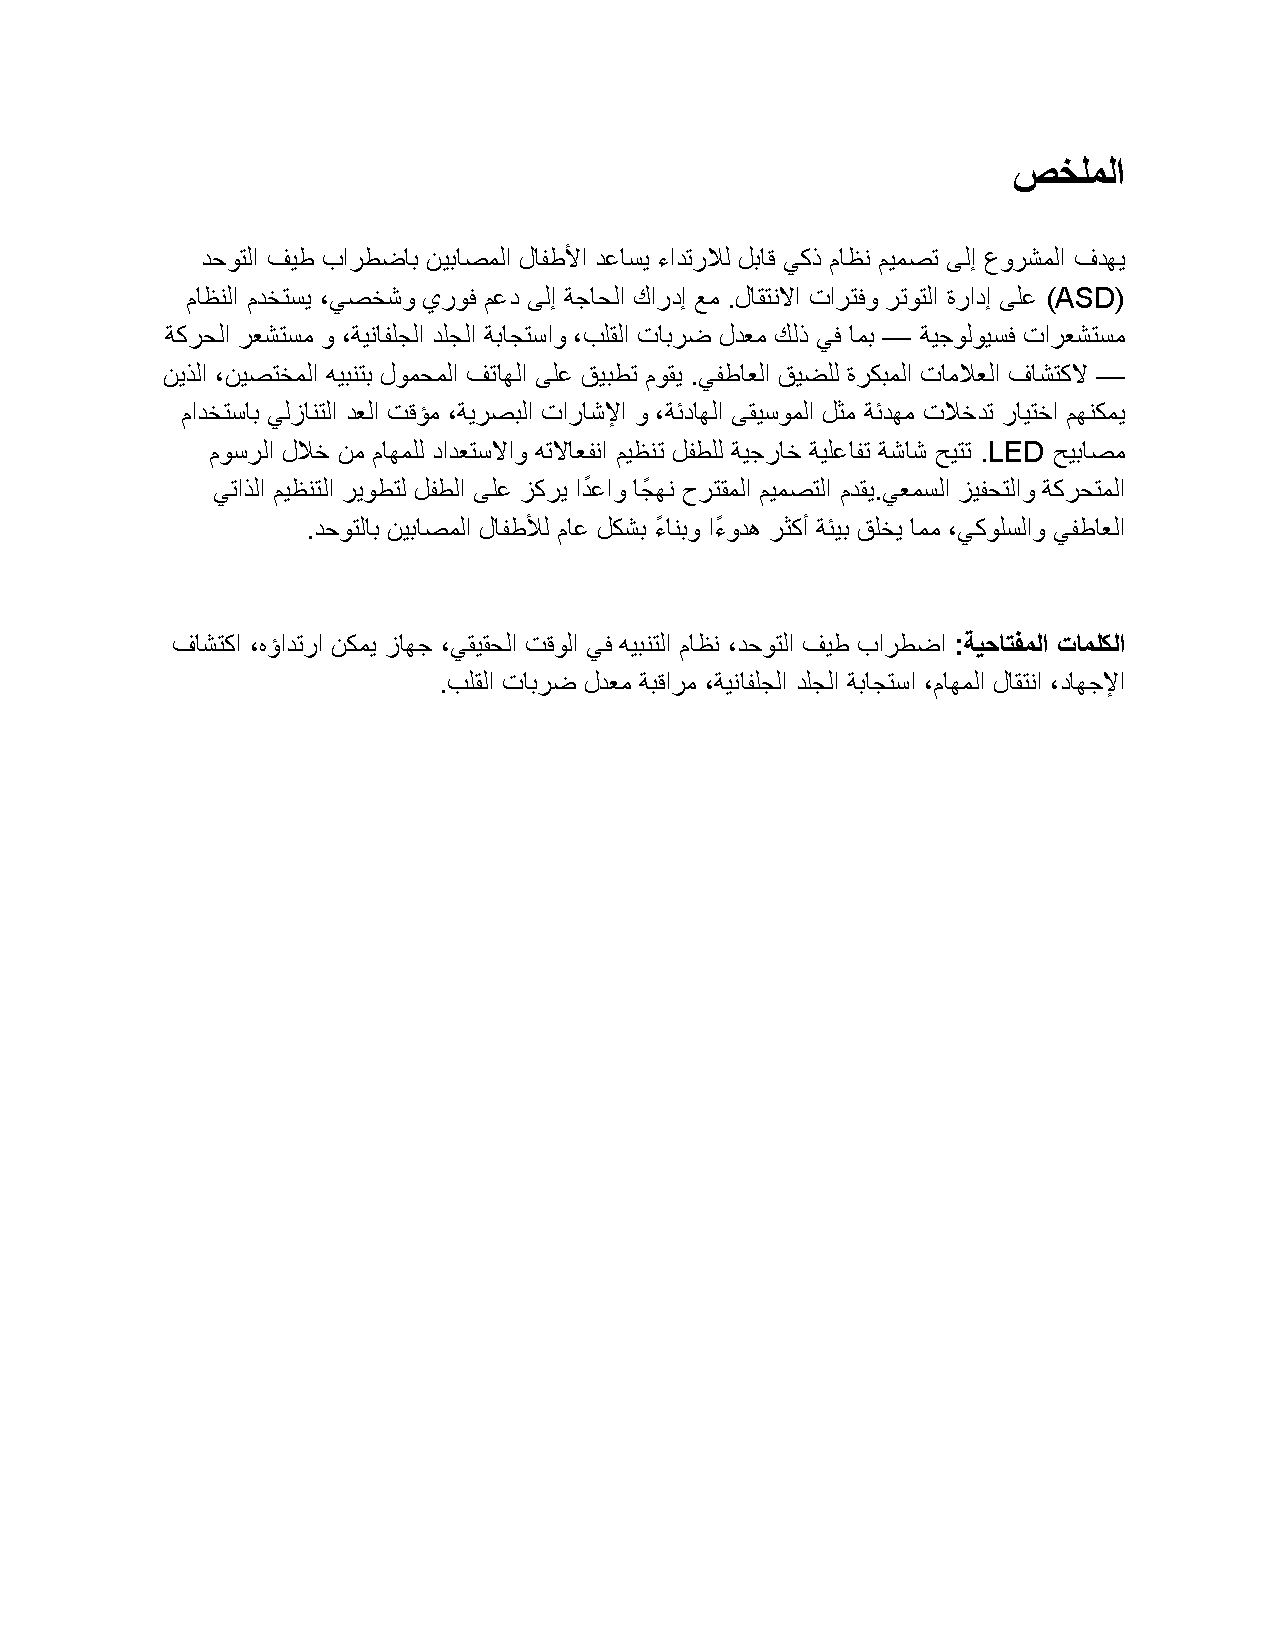
\includepdf[pages=-, pagecommand={\thispagestyle{plain}}]{Abstract.pdf}
\newpage


\chapter{Introduction}

\section{Preface}
The intelligent stress management for children with Autism Spectrum Disorder (ASD) is basically an on the spot personalized support, helping children through their emotional challenges and smoother task transitions. Autistic children become anxious and sometimes disengaged when facing some unexpected change or overwhelming situation, traditional methods like verbal cues or static routines just cannot suffice to meet the need at that very moment.\\[0.5cm]
This system improves emotional well-being by recognizing early signs of stress and providing personalized support to help children stay calm and focused. Advanced monitoring and intervention methods assist children in developing improved adjustment skills that improve their daily social interactions and life quality. In addition, the use of structured visual instruction integration facilitates task execution and reducing anxiety and confusion. At the end, this project is an intriguing this is a tangible way to increase autonomy and build a more leveled, engaging community for autistic children.


\section{Problem Statement}

Children with ASD need support tailored to their needs, helping them express emotion and adjust to stress and transitions between activities. They should receive an immediate personalized intervention according to their needs so that they may be able to lead through activities in a calm transition and supportive environment.\\[0.5cm]
Currently, most support systems use a static approach, bringing in elements such as verbal prompts, picture schedules, or set routines, which can sometimes fail to help when there is a sudden mood change. These negative changes often go unnoticed at first, gradually contributing to stress, frustration, or disengagement in emotions. Without visual cues for changes, transitions from one task to another can be so adversarial that it makes adjustments all the harder.\\[0.5cm]
To overcome these difficulties, the proposed solution helps a smart system to identify early distress signs and intervene with customized real-time responses. Through the means of auditory prompting, sensory feedback, and interactive visual cues, the system stimulates an ambience that helps kids to regulate emotions, lower anxiety, and walk through everyday activities with more confidence and ease.



\section{Project Aims and Objectives}

In this project, we propose a system that aims to provide the following features:

\begin{enumerate}
    \item The system aims to provide real-time emotional support for children with ASD to stress management and emotional self-regulation. In order to complete this aim, the following objectives should be achieved:
    \begin{enumerate}[label=(\alph*)]
        \item Develop a system that continuously monitors the child's emotional and physiological status.
        \item Integrate feedback mechanisms (auditory, sensory, and visual) to provide immediate interventions based on detected stress levels.
        \item Ensuring seamless system component level communication for real-time data exchange.
    \end{enumerate}

    \item The system aims to provide personalized interventions based on the child’s emotional and behavioral responses. In order to complete this aim, the following objectives should be achieved:
    \begin{enumerate}[label=(\alph*)]
        \item Use data analysis techniques for real-time prediction of emotional states and stress levels.
    \end{enumerate}

    \item The system aims to improve task transitions and time management for children with ASD using visual and auditory tools. In order to complete this aim, the following objectives should be achieved: 
    \begin{enumerate}[label=(\alph*)]
        \item Create a visual system that provides transition cues between activities to help children expect changes.
        \item Provide calming auditory and visual cues during transitions. These cues are activated in response to the child’s stress level and are managed by a specialist through a  mobile application to ensure personalized and timely support during routine changes.
    \end{enumerate}
\end{enumerate}

\section{Requirements}

To specify the system requirements, the following functional and non-functional requirements are considered:

\subsection{Functional Requirements}

The system must be able to:
\begin{enumerate}
    \item Identify and track signs of emotional discomfort in autistic children.
    \item Respond immediately through a variety of feedback mechanisms when stress is detected.
    \item Include a structured method to help children transition between activities.
    \item Collect and analyze user data to recognize behavioral patterns and improve actions taken by the system.  
    \item Enable specialists to receive stress alerts and remotely activate personalized interventions via a mobile application.
    \item Operate in real-time, ensuring timely responses to events causing stress.
\end{enumerate}

\subsection{Non-Functional Requirements}

\begin{enumerate}
    \item \textbf{Reliability:}  To minimize false positives and ensure correct actions, the system aims to achieve an accuracy of up to 90\%.
    \item \textbf{Response Time:} To provide immediate assistance, the system aims to respond within about 5 seconds.
    \item \textbf{Usability:} Specialists should be able to easily navigate and use the system interface.
\end{enumerate}

\section{System Description}
Our system is a wearable device can be worn on the child’s hand. It is designed to help children with Autism Spectrum Disorder (ASD) regulate their emotions and manage transitions between tasks. The system consists of sensors and interactional components intended to detect early cues that something is troubling them and provide timely support.\\[0.5cm]
The system consists of three subsystems, a wearable device, an Interactive screen, and mobile application. The wearable device has a heart rate monitor for sensing heart pulse rate and the system can determines heart rate change, a skin conductance sensor to sense the amount of sweat, which is considered an index of stress, and movement sensors that track abnormal movement patterns. All the sensors are reading data in real time, and this is being processed to recognize signs of emotional disturbance. When stress is detected, the system sends an alert that is sent out via a mobile application to the specialist or teacher in real time. Based on the child’s current emotional state and needs, the specialist selects the appropriate calming intervention, such as activating soothing sounds with adjustable volume levels or modifying the intensity of visual feedback like screen brightness. This collaboration provides more specific and individualized regulation strategies, ensuring that assistance is tailored to the child's condition in real time.\\[0.5cm]
To assist in transitioning between activities like transitioning between classes, daily tasks in the classroom, and individual activities to group or reverse activities. the wearable has an LED based countdown timer, which the specialist can configure remotely to help the child prepare for transitions between tasks. This is supplemented by an external interactive screen that can offer calming visual and auditory stimuli, including calming animations, or visually stimulating content to help with emotional regulation. With ongoing monitoring, adaptive feedback, and guided task based instruction, the device demands to impact emotional regulation and daily management routines for children with autism.\\[0.5cm]
\begin{figure}[h]
    \centering
    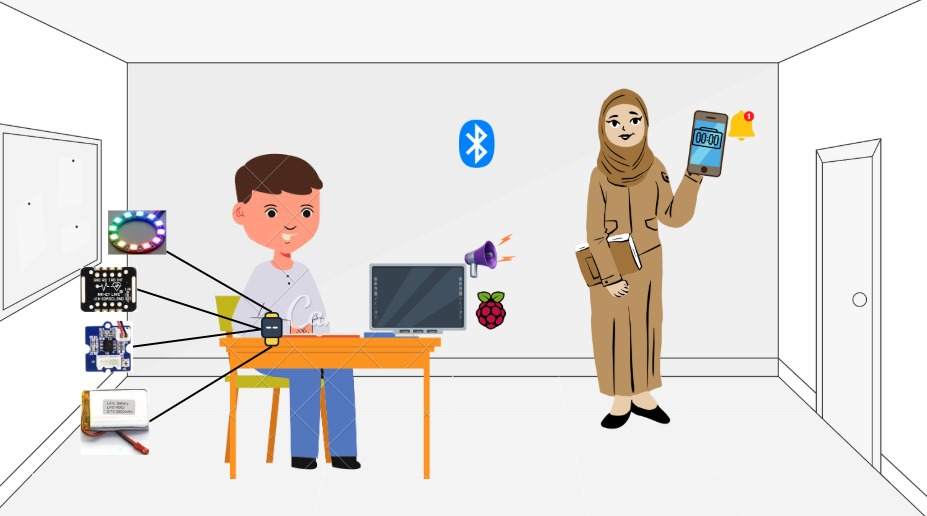
\includegraphics[width=0.6\textwidth]{figure/sysdesc.jpg}
    \caption{System’s Expected Structure}
    \label{fig:system_description}
\end{figure}


\newpage
\section{Project Limitations/Constraints}

\begin{enumerate}

\item \textbf{Cost Constraint:}
Our system model will simulate real life situations for children with Autism Spectrum Disorder (ASD). The proposed solution is designed to simulate the type of support system we will need. However, it will be built using professional components, and the components will be a higher cost. Therefore, and because we are using expensive components we will design the prototype according to what is efficient for our model.
\item \textbf{Wireless Connectivity and Detection Range:}
Communication among wearable device, mobile application for the specialists, and external interactive screen are conducted via wireless communications. Poor wireless communications signal or a child's movement out of range may interrupt communications between devices. Delay in alerts or calming interventions may be caused, hence lowering emotionally rehab's timely effectiveness.
\item \textbf{Power Limitations:}
Since the wearable device runs on battery power, it needs regular recharging. If it isn’t charged in time, the system could temporarily stop monitoring.
\item \textbf{Environmental Factors:}
Environmental factors may affect sensor accuracy, including temperature, humidity, or background noise, which may lessen the reliability of stress detection in some situations.
\item \textbf{Adaptation Time:}
The system requires time to adapt and personalize its responses. For autistic children, adaptation is crucial since they have to get used to wearing the system on their wrist.
\end{enumerate}

\newpage
\section{Schedule}
The tasks of the system implementation and operation are distributed along the first semester, summarized in Table 1.1.

\begin{table}[h] 
    \centering
    \caption{Project Timeline for the First Semester}
    \vspace{0.5em}
    \renewcommand{\arraystretch}{1.3}
    \begin{tabular}{|l|c|c|c|c|}  % أضفنا عمود جديد
        \hline
        \multicolumn{1}{|c|}{\textbf{Task / Week}} & \multicolumn{4}{c|}{\textbf{The First Semester}} \\ \hline
        & \textbf{1 - 4} & \textbf{5 - 10} & \textbf{11 - 15} & \textbf{16 - 20} \\ \hline
        Selection of Project Idea & \cellcolor{gray!30} &  &  &  \\ \hline
        Collecting the Data        &  & \cellcolor{gray!30} & \cellcolor{gray!30} &  \\ \hline
        System Design              &  &  & \cellcolor{gray!30} & \cellcolor{gray!30} \\ \hline
        Documentation              &  & \cellcolor{gray!30} & \cellcolor{gray!30} & \cellcolor{gray!30} \\ \hline
    \end{tabular}
    \label{tab:timeline}
\end{table}


% \begin{table}[h]
%     \centering

%     % العنوان فوق الجدول، يدويًا ومتمركزًا
%     \caption{Project Timeline for the First Semester}

%     \vspace{0.5em}

%     \renewcommand{\arraystretch}{1.3}
%     \begin{tabular}{|l|c|c|c|}
%         \hline
%         \multicolumn{1}{|c|}{\textbf{Task / Week}} & \multicolumn{3}{c|}{\textbf{The First Semester}} \\ \hline
%         & \textbf{1 - 4} & \textbf{5 - 10} & \textbf{11 - 15} \\ \hline
%         Selection of Project Idea & \cellcolor{gray!30} &  &  \\ \hline
%         Collecting the Data        &  & \cellcolor{gray!30} & \cellcolor{gray!30} \\ \hline
%         System Design              &  &  & \cellcolor{gray!30} \\ \hline
%         Documentation              &  & \cellcolor{gray!30} & \cellcolor{gray!30} \\ \hline
%     \end{tabular}

%     % العنوان في caption حتى يظهر في قائمة الجداول
%     \label{tab:timeline}
% \end{table}




\section{Report Outline}

This report is organized as follows: Chapter 2: Provides an overview of definition and classifications for Autism, and sensory processing difficulties in Autistic children, along with a literature review that compares our project to similar ones. Chapter 3: Outlines the project’s design, including both hardware and software aspects. It discusses design choices, the conceptual background of the software, the sequence diagram and presents a schematic diagram.

\chapter{THEORETICAL BACKGROUND}

\section{Preface}

This chapter introduces the theoretical foundation essential to our project. Following this, we will conduct a literature review, comparing our project with previous works related to our work. This comparison will help highlight the unique aspects and innovations our project introduces. In summary, this chapter provides the necessary background to understand the origins of our project and its position within existing research.
\section{Theoretical Background}

This section provides an overview of definition and classifications for Autism, and sensory processing difficulties in Autistic children.

\subsection{Autism Spectrum Disorder (ASD): Definition and Classifications}
\subsubsection{Definition}
Autism is defined according to the Individuals with Disabilities Education Act (IDEA) as a developmental disability having a substantial effect on verbal and nonverbal communication and social interaction, with onset generally before age three, and which adversely affects a child's educational performance.  It is often associated with repetitive behaviors, resistance to change, and unusual sensory responses. If a child shows these traits after age three but meets the criteria, they may still be diagnosed. Qualified professionals, such as psychiatrists or pediatricians, make the diagnosis \cite{specialeducationguide_autism}.

\subsubsection{Classifications}
According to the Diagnostic and Statistical Manual of Mental Disorders, Fifth Edition (DSM-5), ASD is classified as a single diagnosis without subcategories (as opposed to DSM-4), and is further divided into three levels based on the level of support required \cite{behavioralinnovations_types_levels_ASD}.\\[0.3cm]
\textbf{Level 1: Requiring Support} \\[0.3cm]
The diagnosis of an individual with Level 1 Autism Spectrum Disorder (ASD) indicates the mildest form of autism. Individuals are typically verbal, able to form sentences, and engage in simple conversations. However, the above could not be expected to prompt or sustain social interaction, and could be expected to have difficulty with understanding social cues or engaging in small talk. They may not find it easy to initiate or sustain close friendships. They may be uncomfortable or anxious because of a change of routine or transition from one task to another. Although they are mostly independent in many places, they still require support, especially in social situations, to manage their interactions and adapt to changes effectively \cite{behavioralinnovations_types_levels_ASD}. \\[0.3cm]
\textbf{Level 2: Requiring Substantial Support}\\[0.3cm]
The diagnosis of an individual with Level 2 Autism Spectrum Disorder (ASD) has much more severe communication and social deficits than Level 1. Individuals at this level often have problems with both verbal and non-verbal communication, and show much more repetitive behaviors such as flapping, rocking, and skin picking. These behaviors can affect daily work or social operations. Such individuals also have difficulties in adjusting to changes in routine and thus require intensive support in many life areas, including academic, occupational, and social contexts. A principle applied to these behaviors has to be in the best interests of the individual with autism \cite{behavioralinnovations_types_levels_ASD}.  \\[0.3cm]
\textbf{Level 3: Requiring Very Substantial Support}\\[0.3cm]
The diagnosis of an individual with Level 3 Autism Spectrum Disorder (ASD) require very substantial support, as they tend to be the most affected by the condition. They tend to have severe communication difficulties, with limited or no verbal skills and little tendency to respond to social cues or others attempts at making contact. People at this level tend to engage in strong and repetitive behaviors and have extreme difficulty handling changes or alterations in routine; they may exhibit meltdowns, aggression, or self-injury at times and require almost constant supervision and interventions. Because of the immediacy of the effect experienced in nearly all areas of life, people with Level 3 autism need broad and comprehensive support throughout life-in-home, school, health care, and the community \cite{behavioralinnovations_types_levels_ASD}. \\[0.3cm]

\renewcommand{\arraystretch}{1.8}  % زيادة المسافة بين الأسطر
\begin{table}[h]
\centering
\caption{Levels of Support in Autism Spectrum Disorder}
\vspace{0.5em}

\begin{tabular}{|>{\centering\arraybackslash}m{3.5cm}
                |>{\centering\arraybackslash}m{3.8cm}
                |>{\centering\arraybackslash}m{4cm}
                |>{\centering\arraybackslash}m{4.2cm}|}
\hline
\textbf{Feature} &
\makecell {\\ \textbf{Level 1} \\ \small(Requires Support) } &
\makecell{\\ \textbf{Level 2} \\ \small(Requires Substantial \\ Support)} &
\makecell{\\ \textbf{Level 3} \\ \small(Requires Very \\Substantial Support)} \\
\hline

Support Needed & Some support & Substantial support & Very substantial support \\
\hline
\makecell{Language \& \\ Communication} & Can speak, mild difficulties & Noticeable challenges & May be nonverbal or limited verbal communication \\
\hline
Social Interaction & Difficulty with casual conversation and friendships & Difficulty with understanding social cues & Severe impairment in social engagement \\
\hline
\makecell{Repetitive \\ Behaviors } & Present but less intense & Frequent, may disrupt daily functioning & Intense, persistent, may be harmful \\
\hline
Independence & Largely independent & Needs regular assistance & Requires constant supervision \\
\hline
Response to Change & Discomfort with change & Resistance to change & Strong resistance and distress \\
\hline
\end{tabular}
\label{tab:asd_support_levels}
\end{table}

\subsection{Sensory Processing Difficulties in Autistic Children}
Children with Autism Spectrum Disorder (ASD) tend to have Sensory Processing Difficulty (SPD), which influences how they perceive and react to sensory input. Their challenges will be different from one child to another but typically emerge as one or more of the following:

\begin{enumerate}[label=\arabic*.]

\item \textbf{Tactile Defensiveness (Hypersensitivity to Touch)} 

Some children with autism are hypersensitive to touch, and even slight contact---such as seams in clothes, wristbands, or nubby fabrics---can be uncomfortable, irritating, or even painful. This sensitivity, known as tactile defensiveness, is one of the most critical considerations in wearable system design.

To address this challenge, it is essential to employ soft, breathable, hypoallergenic materials in any wearable component, and to render the device light, pliable, and easy to adjust. However, comfort may not suffice to guarantee effective adoption.

Kientz et al.\ (2020) investigated how autistic children perceive wearing a smartwatch. Some children tolerated the smartwatch after receiving simple verbal guidance, but others initially refused it due to discomfort. Interestingly, the study demonstrated the effectiveness of their method, which was based on visual schedules with video modeling that visually broke down the process of wearing the watch into small, manageable steps. This gradually increased tolerance: 62.5\% of the participants (5 out of 8) later wore the smartwatch comfortably while also engaging in related activities \cite{obrien2020_smartwatch_ASD}.

This suggests that gradual, structured exposure can reduce tactile defensiveness, improving acceptance of wearables in children with ASD. Moreover, material selection and introduction strategies significantly influence successful adoption, emphasizing their impact on intervention approaches.

\item \textbf{Hypo-responsiveness (Under-Responsiveness)}

Some ASD children do not react much to physical stimulation. They will not notice a watch on their wrist, may not register important notifications (e.g., vibrations), or will not sense discomfort due to an incorrectly fitting device. In these cases, it is helpful to add multi-sensory feedback (e.g., visual notification, light vibration, or audio notification) to make the device more noticeable and effective.

\item \textbf{Sensory Seeking Behaviors}

Unlike defensiveness, other children actively seek out sensory input. They might like to make physical contact, touch, or move and might even find the watch soothing or stimulating. For these children, wearables can be developed with self-regulating calming sensory feedback, such as vibrations, smooth texture, or visual animations.

\end{enumerate}

\clearpage
\begin{table}[h]
\centering
\caption[Comparison of Sensory Processing Difficulties in Autistic Children]{Comparison of Sensory Processing Difficulties in Autistic Children \cite{autismorg_uk_sensory_differences}.}

\renewcommand{\arraystretch}{1.2} % زيادة المسافة بين الأسطر
\begin{tabular}{|p{3.2cm}|p{4.5cm}|p{4cm}|p{4.2cm}|}
\hline
\textbf{Category} & \textbf{Common Behaviors} & \textbf{Real-life Examples} & \textbf{Support Strategies} \\
\hline
\textbf{Over-Responsiveness} &
\begin{itemize}[leftmargin=*, nosep]
  \item Pain from light touch.
  \item Dislike of certain fabrics.
  \item Hair washing difficulties.
  \item Food texture sensitivity.
\end{itemize} &
\begin{itemize}[leftmargin=*, nosep]
  \item Refuses tight clothing.
  \item Cries when head is touched.
  \item Eats limited foods.
\end{itemize} &
\begin{itemize}[leftmargin=*, nosep]
  \item Warn before touching
  \item Remove clothing labels
  \item Gradual texture exposure using soft tools
\end{itemize} \\
\hline
\textbf{Under-Responsiveness} &
\begin{itemize}[leftmargin=*, nosep]
  \item High pain threshold
  \item Doesn’t notice food in mouth
  \item Chews on non-food items
  \item Seeks deep pressure
\end{itemize} &
\begin{itemize}[leftmargin=*, nosep]
  \item Hugs too tightly
  \item Bites or hits self
  \item Loves heavy blankets
\end{itemize} &
\begin{itemize}[leftmargin=*, nosep]
  \item Provide safe chew alternatives
  \item Use weighted items
  \item Offer structured sensory activities
\end{itemize} \\
\hline
\textbf{Sensory Seeking }&
\begin{itemize}[leftmargin=*, nosep]
  \item Rubs textures
  \item Seeks vibrations
  \item Enjoys spinning or movement
\end{itemize} &
\begin{itemize}[leftmargin=*, nosep]
  \item Touches walls frequently
  \item Jumps or spins constantly
  \item Craves tight hugs
\end{itemize} &
\begin{itemize}[leftmargin=*, nosep]
  \item Provide sensory-rich toys
  \item Integrate vibration safely
  \item Include sensory input in routines
\end{itemize} \\
\hline
\end{tabular}
\label{tab:sensory_behaviors}
\end{table}

% \clearpage
% \renewcommand{\arraystretch}{1.8}  % زيادة المسافة بين الأسطر
% \begin{table}[h]
% \centering
% \caption{Comparison of Sensory Processing Difficulties in Autistic Children}
% \vspace{0.5em}

% \begin{tabular}{|>{\centering\arraybackslash}m{3.2cm}
%                 |>{\centering\arraybackslash}m{4.2cm}
%                 |>{\centering\arraybackslash}m{4.2cm}
%                 |>{\centering\arraybackslash}m{4.2cm}|}
% \hline
% \textbf{Category} &
% \textbf{Common Behaviors} &
% \textbf{Real-life Examples} &
% \textbf{Support Strategies} \\
% \hline

% \makecell{\textbf{Over-}\\\textbf{Responsiveness}}& 
% \makecell{
% - Pain from light touch\\
% - Dislike of certain fabrics\\
% - Hair washing difficulties\\
% - Food texture sensitivity
% } & 
% \makecell{- Refuses tight clothing\\- Cries when head is touched\\- Eats limited foods
% } & 
% \makecell{- Warn before touching\\
% - Remove clothing labels\\
% - Gradual texture exposure using soft tools \\} \\
% \hline

% \makecell{\textbf{Under-}\\\textbf{Responsiveness}} &
% \makecell{
% - High pain threshold\\
% - Doesn’t notice food in mouth\\
% - Chews on non-food items\\
% - Seeks deep pressure 
% } &
% \makecell{
% - Hugs too tightly\\
% - Bites or hits self\\
% - Loves heavy blankets 
% } & 
% \makecell{
% - Provide safe chew alternatives\\
% - Use weighted items\\
% - Offer structured sensory activities 
% }\\
% \hline


% \makecell{\textbf{Sensory}\\\textbf{Seeking}} &
% \makecell{
% - Rubs textures\\
% - Seeks vibrations\\
% - Enjoys spinning or movement\\
% } &
% \makecell{
% - Touches walls frequently \\
% - Jumps or spins constantly\\
% - Craves tight hugs 
% } &
% \makecell{
% - Provide sensory-rich toys\\
% - Integrate vibration safely\\
% - Include sensory input in routines 
% }\\
% \hline
% \end{tabular}
% \label{tab:sensory_processing_categories}
% \end{table}

\section{Literature Review}
Recent projects have explored wearable and assistive technologies to support autistic children, focusing on stress detection, communication, and behavior management. This section reviews key examples from past work to compare their features and limitations with our proposed system.
\subsection{Preventing, Anticipating and Mitigating Off-Task Behavior in Special Needs Students}
Authors in this work \cite{ucf_offtask_behavior_project} aimed to help children with transitioning difficulties related to Autism Spectrum Disorder (ASD) or Emotional Behavior Disorder (EBD) in transitioning from one school activity to another while reducing the occurrence of off-task behaviors that may interfere with learning. The project includes the implementation of a wearable sensor system, which has the Atmega328P microcontroller programmed via Arduino Integrated Development Environment  (IDE), meant to collect physiological markers-stress symptoms in terms of heart rate, temperature, and sweating. It incorporates an LED-based countdown timer for upcoming changes and a touchscreen device for giving students calming activities intended to help them handle sensory overload. The project created an effective operational system that real-time-notifies teachers so the pupils would have early intervention; however, challenges include sensor accuracy, as sometimes readings are affected by the environment, and how to engage the interactive device yet prevent distraction from learning. It also needs further study regarding which way should LED countdown be set-on a period basis or time basis. With all these challenges, this project will establish a very good basis to improve the classroom experience for children with ASD and EBD. 

\newpage
\subsection{Empatica E4 Wristband}
The authors in \cite{empatica_EmbracePlus} describe the E4 as a wearable physiological monitoring device designed for continuous, real-time health monitoring in medical and research applications. It provides non-invasive measurement of significant physiological signals including electrodermal activity (EDA), heart rate variability (HRV), skin temperature, and motion activity, and is therefore applicable to the study of stress, emotional responses, neurological diseases, and well-being. With the utilization of advanced biosensors such as photoplethysmography (PPG), infrared thermopile, 3-axis accelerometer, and Bluetooth, the device enables real-time data streaming and cloud-based analysis through Empatica's software platforms. The E4 has widely been used in science research and clinical trials, offering high-quality physiological data for mental illness, sleep research, and stress monitoring. However, costs are high (\$1,690), short battery life, and reduced EDA consistency, which are disadvantages in part for this. It has also been discontinued. However, it has made a really good contribution to the strides made in wearable health monitoring, and lays the foundation for innovations in biometric tracking in the future.

\subsection{New Tool for Kids \& People with Autism: The Gizmo Watch 3 - Adventure}
The authors in \cite{verizon_GizmoWatch3_Autism} introduced the Gizmo Watch 3 has been introduced by Verizon and the Autism Society of America for building independence, communication, and security for children and individuals with Autism. Now, the smartwatches boast of GPS tracking and geofencing for reporting location in real-time monitoring, voice-to-text messaging, programmable timers, and reminders for giving a soft touch to everyday activity routines. They are really programmed to encourage a kid's physical activity by step counting and jumping, even offering special games designed for neurodivergent kids. They have shown a lot of potential to make quite an impact on the management of routine activities, safety, and certainly controlled communication through a sturdy design for rough handling. One such hitch, however, is discomfort for sensory-sensitive children and rather limited texting for older users too, requiring more advanced tools for communication. On neither of these counts can Gizmo Watch 3 be considered a medical device. Children with Autism can use such smart applications for the relevant purposes of building structured independence, safety, and an engaging but user-friendly way of living.


\clearpage
A summary of the comparison is presented in Table 2.3 .

\renewcommand{\arraystretch}{1.8} % زيادة المسافة بين الأسطر
\begin{table}[h]
\centering
\small
\caption{Comparison with other projects}
\vspace{0.5em}

\begin{tabular}{|>{\centering\arraybackslash}m{3cm}
                |>{\centering\arraybackslash}m{3.5cm}
                |>{\centering\arraybackslash}m{3cm}
                |>{\centering\arraybackslash}m{3cm}
                |>{\centering\arraybackslash}m{3.5cm}|}
\hline
\textbf{Feature} &
\makecell{\textbf{Preventing } \\ \textbf{Anticipating} \\ \textbf{\& Mitigating} \\ 
\textbf{Off-Task} \\ \textbf{Behavior in} \\ 
\textbf{Special Needs}\\  \textbf{Students}} &
\makecell{\textbf{Empatica E4 } \\ \textbf{Wristband}} &
\makecell{\textbf{The Gizmo } \\ \textbf{Watch} \\ \textbf{3 - Adventure}} &
\makecell{\textbf{Our Project}} \\
\hline

\textbf{Device Type} &
Wearable + Interactive Screen &
Medical-grade wristband &
Smartwatch for kids &
Wearable wristband + external interactive screen \\
\hline

\textbf{Target Group} &
Children with ASD or EBD &
Patients, research subjects &
Children with Autism &
Children with Autism Spectrum Disorder \\
\hline

\textbf{Main Goals} &
Reduce off-task behaviors and ease activity transitions &
Continuous physiological monitoring for stress and health &
Promote independence, safety, and communication &
Provide real-time emotional support and smoother task transitions \\
\hline

\textbf{Sensor Types} &
Heart rate, temperature, sweat (stress indicators) &
EDA, HRV, temperature, accelerometer &
Basic motion sensor &
Heart rate, sweat (EDA), motion sensors \\
\hline

\textbf{Limitations} &
Environmental sensor sensitivity, possible distraction &
Very high cost, short battery life, discontinued &
Not a medical device, limited texting, may irritate sensory-sensitive kids &
Cost, Bluetooth range, battery, environment, adaptation time\\
\hline

\textbf{Cost} &
\$40–80 (prototype-based) &
\$1,690 &
\$150 (device only) &
To be determined later\\
\hline

\end{tabular}
\label{tab:device_comparison}
\end{table}

Unlike past projects concentrating on monitoring or basic alerts, Our system integrates real-time emotional detection with guided professional support.It includes a wearable wristband equipped with GSR and heart rate sensors to monitor stress indicators, and an external interactive screen where the specialist can display calming visuals and auditory cues relevant to the child's current emotional state.
The system involves the specialist in interpreting information and giving the most appropriate response, rendering the support sensitive to the sensory profile of every child. A visual countdown through an LED ring helps to facilitate transitions between tasks, with the system being cost effective, school friendly, and easily adaptable to the specific needs of autistic children. This adaptive integration of feedback, real time data, and human intervention distinctly separates our project from existing solutions.

\section{Summary}
In this chapter, we presented the theoretical background needed to understand the key aspects of our project, i.e., stress detection, machine learning, real-time processing of data, decision-making algorithms, and HCI guidelines. We also conducted a literature review where we compared our system with similar existing projects. The comparison outlines how our project stands out by merging real-time emotional detection with interactive, personalized support through both a wearable device and an external screen, especially for children with autism.  

\chapter{ SYSTEM DESIGN}
\section{Preface}
This chapter provides an overview of the necessary hardware and software components intended for our project. It explores various options for each component, presents a conceptual description of the system, and launches a general block diagram. Additionally, the chapter delves into system algorithms and methodologies through the use of flowcharts. Schematic diagrams depict the interactions and interfaces between components.
\section{ System components and Design alternatives}
This part describes the hardware and software components and their design alternatives.
\subsection{Hardware Components}
\subsubsection{Wearable Device}
The wearable unit is responsible for detecting physiological stress signs from the child, processing them, and providing sensory feedback.
\paragraph{Microcontroller \\[0.3cm]}
The microcontroller is a main component in the wearable device, which collects physiological data from sensors and controls feedback output such as visual cues. There are three available options for the microcontroller ESP-WROOM-32, LilyPad Arduino, and Raspberry Pi Zero W to choose from shown in Table 3.1.

\clearpage
\renewcommand{\arraystretch}{1.8} % زيادة المسافة بين الأسطر

\begin{table}[h]
\centering
\caption{ Differences between ESP-WROOM-32, LilyPad Arduino, and Raspberry Pi Zero W}
\vspace{0.5em}

\begin{tabular}{|>{\centering\arraybackslash}m{3.5cm}
                |>{\centering\arraybackslash}m{3.5cm}
                |>{\centering\arraybackslash}m{3.5cm}
                |>{\centering\arraybackslash}m{3.5cm}|}
\hline
\textbf{Characteristic} & \textbf{ESP-WROOM-32 \cite{xecor_esp32_vs_arduino}} & \textbf{LilyPad Arduino \cite{makerstore_LilyPad_Mboard}} & \textbf{Raspberry Pi Zero W \cite{cytron_raspi_zero2w}} \\
\hline

\textbf{Image} &
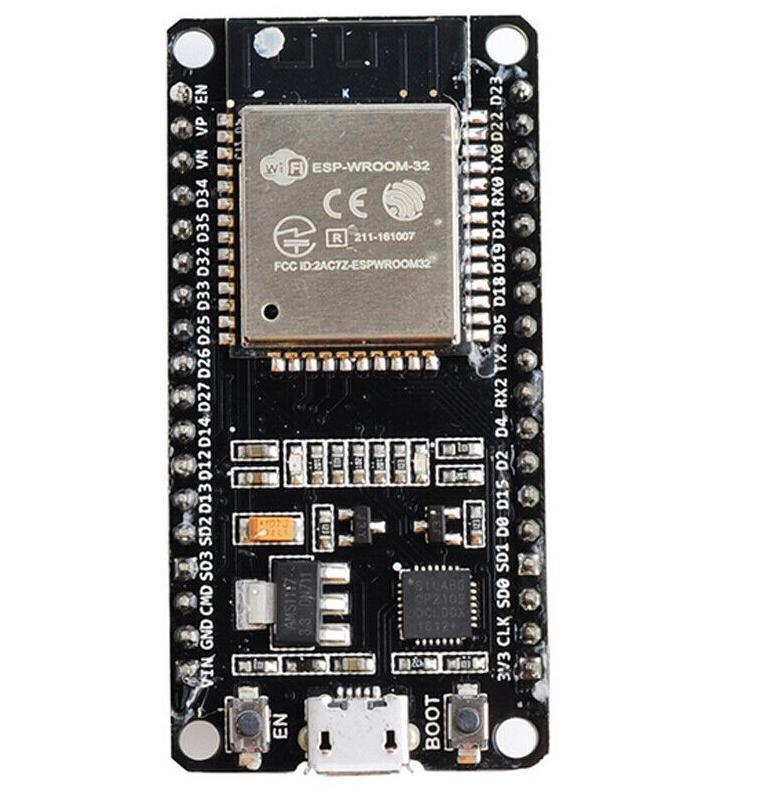
\includegraphics[width=2.5cm]{figure/ESP32 WROOM.jpg} &
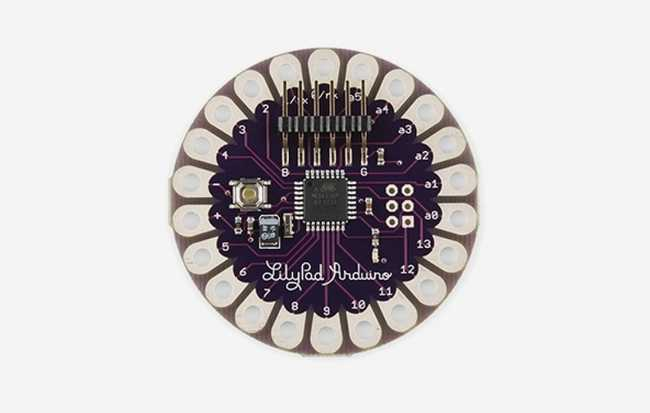
\includegraphics[width=2.5cm]{figure/lilypad-arduino.jpg} &
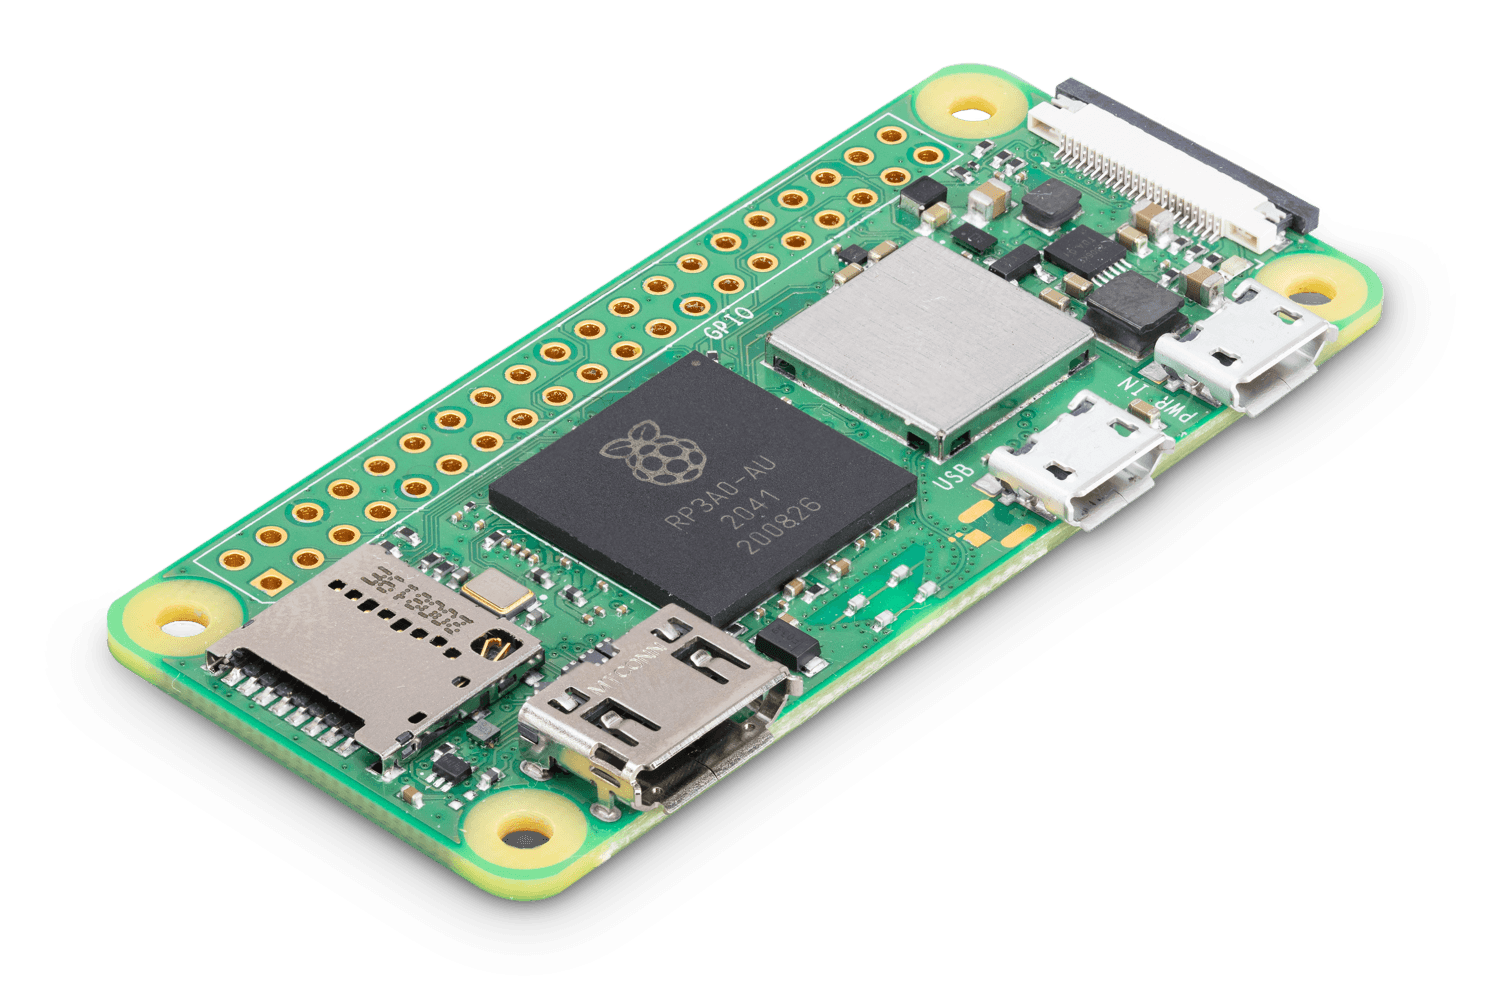
\includegraphics[width=2.5cm]{figure/raspberry pi zero.png} \\
\hline

\textbf{RAM} &
520KB SRAM &
1KB SRAM &
512MB \\
\hline

\textbf{Clock Speed} &
Up to 240MHz &
8 MHz &
1GHz \\
\hline

\textbf{Storage} &
Up to 16MB Flash &
16 KB &
microSD \\
\hline

\makecell{\textbf{Dimensions} \\ \textbf{(L x W x H) mm}} &
(18mm $\times$ 25.5mm $\times$ 2.8mm) \cite{nabto_iot_esp32} &
approximately 50mm diameter, height 4.5mm &
(65mm $\times$ 30mm $\times$ 13mm) \\
\hline

\textbf{Connectivity} &
WiFi, Bluetooth &
No built-in WiFi/Bluetooth &
WiFi, Bluetooth \\
\hline

\textbf{Price} &
starts from around \$4 &
starts from \$1 -- \$3 \cite{alibaba_lilypad328} &
from \$35 -- \$75 \\
\hline

\textbf{Operating Voltage} &
3.0V--3.3V &
2.7V--5.5V &
5V via micro-USB \\
\hline

\end{tabular}
\label{tab:microcontrollers_comparison}
\end{table}

The ESP-WROOM- 32 was chosen because it’s speed, large memory and built-in WiFi/Bluetooth, making it ideal for real-time sensor data processing and wireless communication in the wearable system.
\paragraph{Skin Conductance Sensors \\[0.3cm]} 
Skin conductance is a standard psychophysiological measurement procedure, often referred to as Electrodermal Activity (EDA). It is used as an index of the activity of the sympathetic nervous system, whose role is to generate the body's response, a physiological response triggered by emotionally arousing or stressful stimuli. \\[0.1cm]

This response increases sweat gland activity, particularly in areas with a high density of sweat glands, such as the fingers and palms. As emotional or psychological arousal rises, such as during stress or anxiety, the skin's ability to conduct electricity improves due to the increased sweat production \cite{mcilwain2019_autism_healthcare}. During stress, the resistance of the skin drops due to increased secretion in the sweating glands \cite{lord2016_autism_diagnosis}. There are two available options for skin conductance sensors to choose from shown in Table 3.2.
\clearpage
\renewcommand{\arraystretch}{1.8} % زيادة المسافة بين الأسطر

\begin{table}[h]
\centering
\caption{Differences between the Grove Galvanic Skin Response (GSR) sensor \newline and Galvanic Skin Response (GSR) Shimmer3 sensor}
\vspace{0.5em}

\begin{tabular}{|>{\centering\arraybackslash}m{4cm}
                |>{\centering\arraybackslash}m{4cm}
                |>{\centering\arraybackslash}m{4cm}|}
\hline
\textbf{Characteristic} & 
\textbf{Grove GSR \cite{seeedstudio_gsr_sensor}} & 
\textbf{GSR Shimmer3 \cite{imotions_shimmer3_gsr}} \\
\hline

\textbf{Image} &
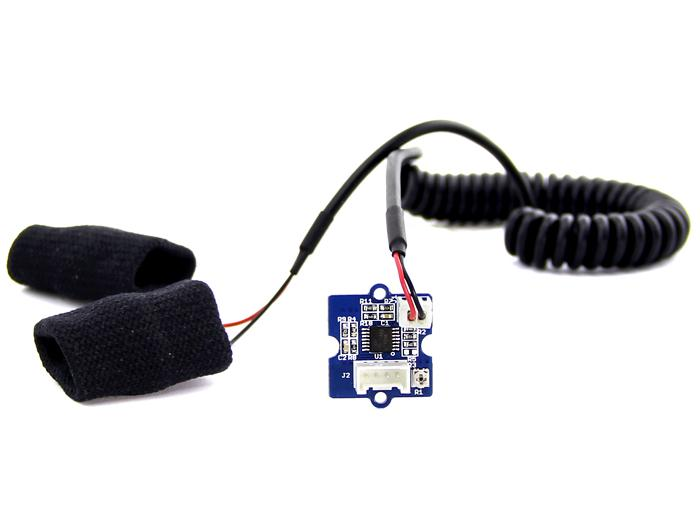
\includegraphics[width=2.5cm]{figure/Grove GSR.jpg} &
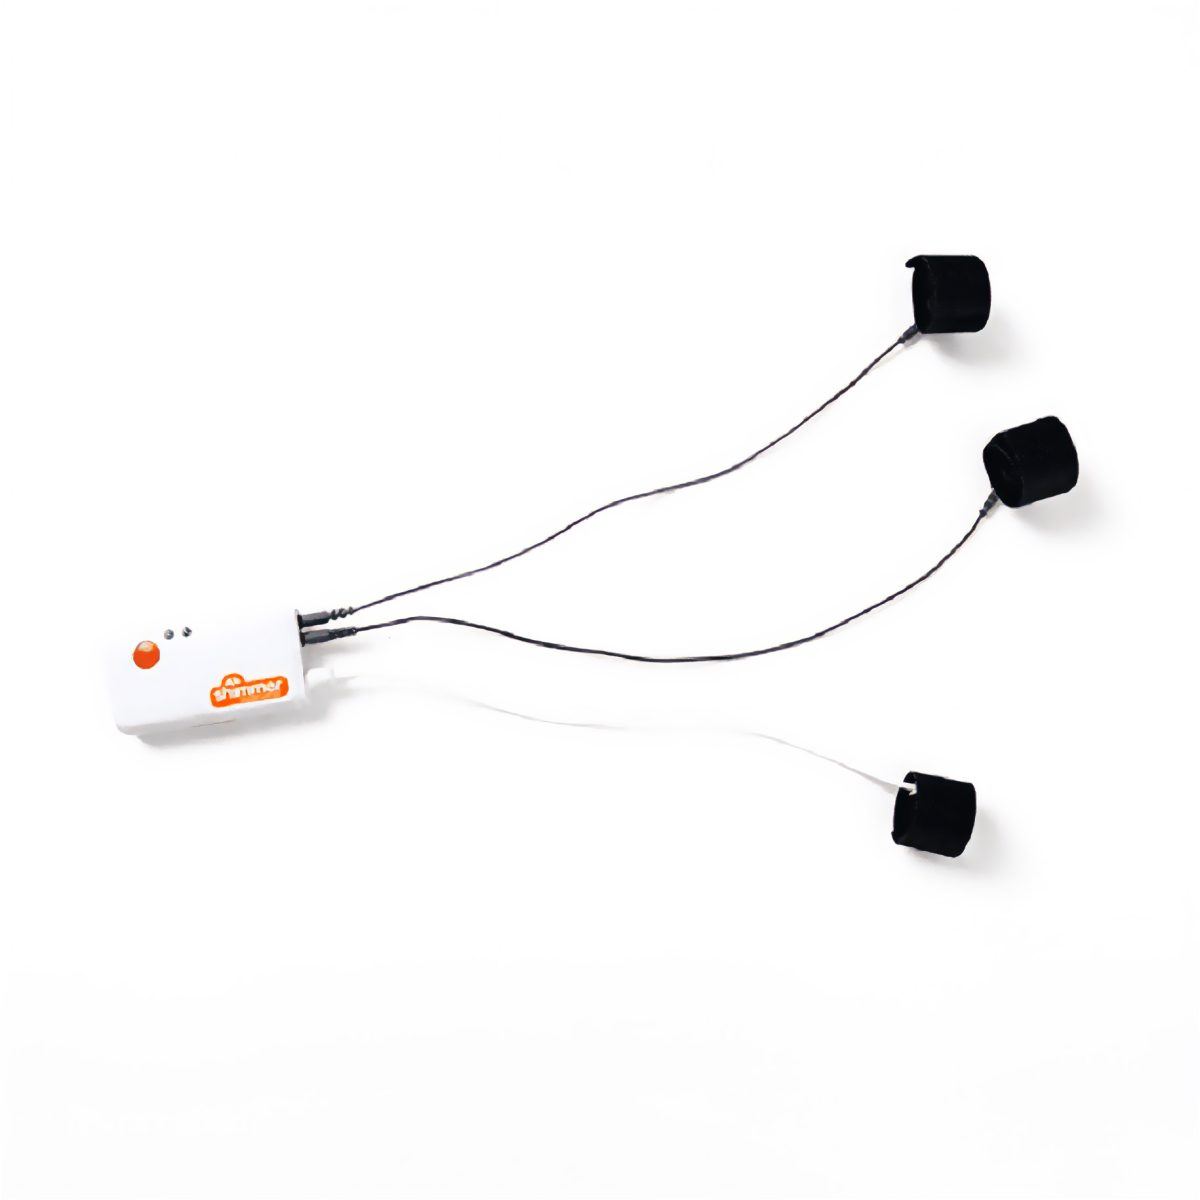
\includegraphics[width=2.5cm]{figure/Shimmer3-GSR.jpg} \\
\hline

\textbf{Price} &
$\approx\$60$--\$70 &
$\approx\$570$ \\
\hline

\textbf{Power Supply} &
Operates at 3.3V / 5V &
Rechargeable 450mAh Li-ion battery + Bluetooth \\
\hline

\textbf{Connectivity} &
Wired (analog output) &
Wireless via Bluetooth / USB / SD card \\
\hline

\makecell{\textbf{Size \&} \\ \textbf{Weight}} &
Very small and lightweight &
Small size, lightweight (28g) \\
\hline

\end{tabular}
\label{tab:skin_conductance_sensors}
\end{table}

The Grove GSR sensor was chosen due to its affordable price, simple integration process, and compatibility with low-power wearable systems. While premium options like the Shimmer3 GSR offer advanced features and medical-grade precision, the Grove GSR provides enough data resolution for detecting stress related physiological changes, which is the main requirement of the system. Additionally, its compact size and minimal energy requirements make it ideal for embedding within a lightweight wearable device.

\paragraph{Heart Rate Sensor \\[0.3cm]}
A heart rate sensor is used to monitor the number of heartbeats per minute (BPM). It provides valuable data into a person’s physiological and emotional state, especially in response to stress, anxiety, or physical activity. In wearable health devices, heart rate monitoring helps in detecting abnormal patterns, and assessing stress levels.There are two available options for heart rate sensors to choose from shown in Table 3.3.

\clearpage
\renewcommand{\arraystretch}{1.8} % زيادة المسافة بين الأسطر

\begin{table}[h]
\centering
\caption{Differences between the MAX30102 sensor and Pulse sensor}
\vspace{0.5em}

\begin{tabular}{|>{\centering\arraybackslash}m{4cm}
                |>{\centering\arraybackslash}m{4cm}
                |>{\centering\arraybackslash}m{4cm}|}
\hline
\textbf{Characteristic} & 
\textbf{MAX30102 \cite{ielectrony_max30102}} & 
\textbf{Pulse Sensor \cite{kitsguru_heartbeat_sensor}} \\
\hline

\textbf{Image} &
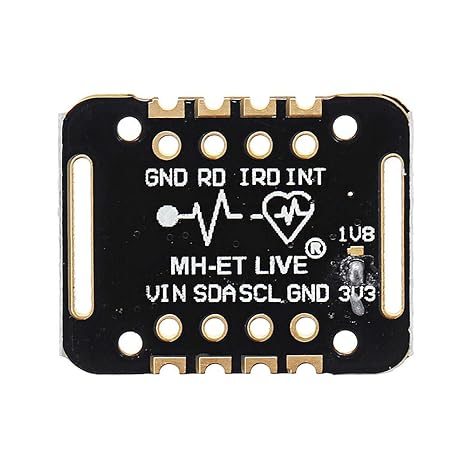
\includegraphics[width=2.5cm]{figure/MAX30102.jpg} &
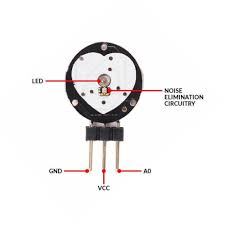
\includegraphics[width=2.5cm]{figure/pulse sensor.jpeg} \\
\hline

\textbf{Price} &
Starts from \$7 &
Starts from \$1 \\
\hline

\textbf{Output Type} &
Digital signal (data stream over I2C) &
Analog voltage (pulse waveform) \\
\hline

\makecell{\textbf{Type of} \\ \textbf{Measurement}} &
Digital biosensor with SpO$_2$ + HR detection &
Analog optical heart rate sensor \\
\hline

\textbf{Detection Method} &
Optical reflection (PPG) with dual-wavelength absorption &
Optical reflection (PPG) with single wavelength \\
\hline

\textbf{Power Control} &
Software-controllable (can be turned off) &
Always on when powered \\
\hline

\textbf{Pin Count} &
7 pins (VIN, GND, SCL, SDA, INT, RD, IRD) &
3 pins (VCC, GND, A0) \\
\hline

\textbf{Weight} &
20g &
Very lightweight \\
\hline

\end{tabular}
\label{tab:heart_rate_sensors}
\end{table}

The MAX30102 sensor module was chosen for this project due to its high accuracy and ability to capture both heart rates and blood Oxygen saturation (SpO2). The physiological signals formed by these parameters are among the prime indicators of stress and emotional states, which correspond directly to the goal of the system, that is, to monitor emotional response in children. MAX30102 differs from other ordinary pulse sensors in having superior noise rejection and ambient light suppression, thus being qualified for wearable applications where reliability and accuracy are crucial.	

\paragraph{Motion Sensor ((MPU6050), (ADXL335)) \\[0.3cm]}
A motion sensor can be used to track the movement, position, or rotation of the body. It is important in monitoring systems such as wearables because it tracks the level of activity, identifies normal and abnormal repetitive motions, as well as differentiates between stress and usual physical responses.There are two available options for motion sensors to choose from shown in Table 3.4.
\clearpage
\renewcommand{\arraystretch}{1.8} % زيادة المسافة بين الأسطر

\begin{table}[h]
\centering
\caption{Differences between the MPU6050 sensor and ADXL335 sensor}
\vspace{0.5em}

\begin{tabular}{|>{\centering\arraybackslash}m{4cm}
                |>{\centering\arraybackslash}m{4cm}
                |>{\centering\arraybackslash}m{4cm}|}
\hline
\textbf{Characteristic} & 
\textbf{MPU6050 \cite{electronicwings_mpu6050}} & 
\textbf{ADXL335 \cite{electronicwings_adxl335}} \\
\hline

\textbf{Image} &
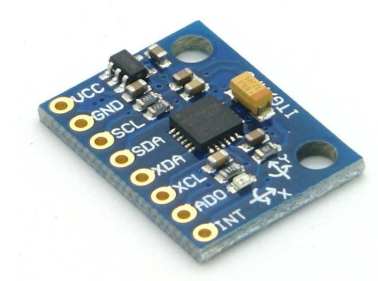
\includegraphics[width=2.5cm]{figure/MPU6050.png} &
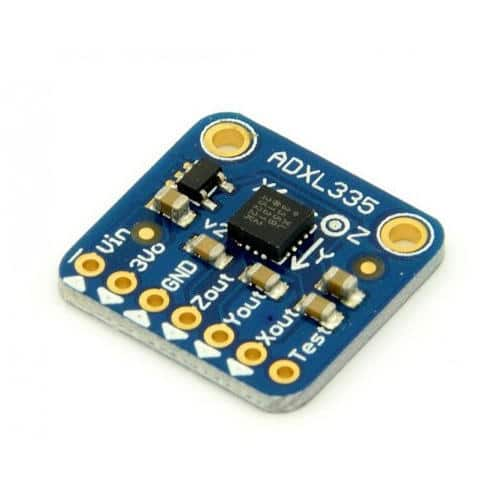
\includegraphics[width=2.5cm]{figure/adxl335.jpg} \\
\hline

\textbf{Price} &
Starts from \$3--5 &
Starts from \$4--6 \\
\hline

\textbf{Sensor Type} &
Digital Accelerometer + Gyroscope &
Analog Accelerometer \\
\hline

\textbf{Axis} &
6 (Accel + Gyro) &
3 (X, Y, Z) \\
\hline

\end{tabular}
\label{tab:motion_sensors_comparison}
\end{table}

The MPU6050 was chosen for this project because it combines a 3-axis accelerometer, 3-axis gyroscope, and an embedded Digital Motion Processor (DMP) in a compact, low-power module.This sensor provides acceleration, orientation, and angular velocity data in all dimensions, making it highly accurate in motion tracking. These motion parameters are essential for detecting physical behaviors and movement patterns that are often stressed in fragile groups of non-aggressive children with autism, such as repeated motions or certain unusual postures of the body.
\paragraph{Display \\[0.3cm]}
An addressable LED strip is used as a visual countdown timer to support emotional self-regulation for children with autism. The LED strip is a non-verbal and intuitive method to indicate time duration, such as for breaks and transitions. The LED strip offers both flexibility in visual design and a strong sensory impact, which can help reduce anxiety during routine changes. There are two available options for  LED strips to choose from shown in Table 3.5.

\clearpage
\renewcommand{\arraystretch}{1.8} % زيادة المسافة بين الصفوف

\begin{table}[h]
\centering
\caption{Differences between the WS2812 NeoPixel Ring and APA102}
\vspace{0.5em}

\begin{tabular}{|>{\centering\arraybackslash}m{4cm}
                |>{\centering\arraybackslash}m{4cm}
                |>{\centering\arraybackslash}m{4cm}|}
\hline
\textbf{Characteristic} & 
\textbf{WS2812 NeoPixel Ring \cite{suntechlite_apa102_vs_ws2812b}} & 
\textbf{APA102 \cite{suntechlite_apa102_vs_ws2812b}} \\
\hline

\textbf{Image} &
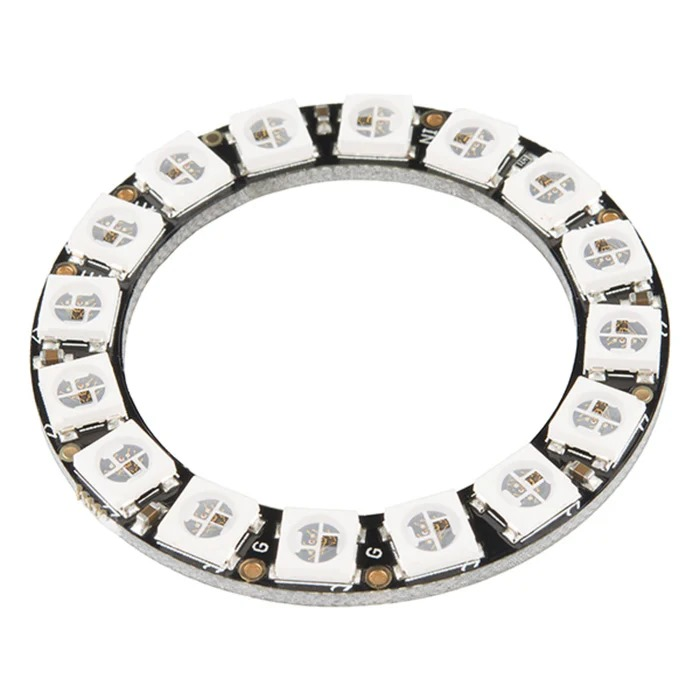
\includegraphics[width=2.5cm]{figure/LED2.jpg} &
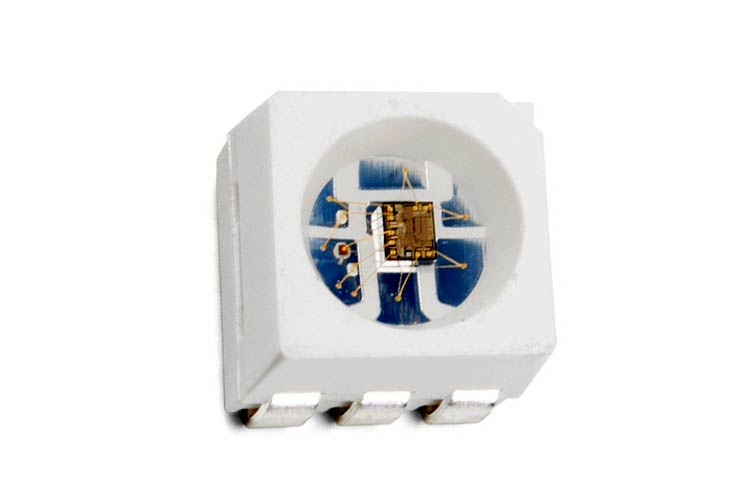
\includegraphics[width=2.5cm]{figure/APA102-RGB-LED.jpg} \\
\hline

\textbf{PWM Resolution} &
8-bit (256 levels) &
8-bit (256 levels) \\
\hline

\textbf{PWM Frequency} &
400 Hz &
20 KHz \\
\hline

\textbf{Type} &
RGB 5050 Pixel &
RGB 5050 or 2020 (Dotstar Micro) Pixel \\
\hline

\textbf{Data Rate} &
800 Kbps &
less than 4 Mbps \\
\hline

\end{tabular}
\label{tab:led_pixel_rings}
\end{table}

The WS2812 NeoPixel Ring was chosen for this project because of its simple integration and for being easily suited for visual feedback applications. It requires only one data line, fully complies with the ESP-WROOM-32 microcontroller, which is going to be used in the project, and prompts bright, individually addressable RGB LEDs \cite{suntechlite_apa102_vs_ws2812b}.

\paragraph{Battery \\[0.3cm]}
For this project, a Lithium-Ion (Li-ion) battery was selected due to its superior energy density, safety profile, and cycle longevity, which are critical for wearable and healthcare-related applications.
 \subsubsection{Interactive Screen}
 Interactive screen is used to present calming audio and visual content to the child under stressful emotional conditions. The screen is also used as a feedback system associated with the wearable device, and it processes incoming data received and responds accordingly. 

\paragraph{Microcontroller \\[0.3cm]} 
The microcontroller of the interactive screen takes input in the form of processed physiological data from the wearable device and displays appropriate visual, auditory, or multimedia data depending upon the emotional state of the child. 
There are two available options for microcontrollers to choose from shown in Table 3.6.

\clearpage
\renewcommand{\arraystretch}{1.8} % زيادة المسافة بين الصفوف

\begin{table}[h]
\centering
\caption{Differences between Raspberry Pi 4B, NVIDIA Jetson Nano}
\vspace{0.5em}

\begin{tabular}{|>{\centering\arraybackslash}m{4cm}
                |>{\centering\arraybackslash}m{4cm}
                |>{\centering\arraybackslash}m{4cm}|}
\hline
\textbf{Characteristic} &
\textbf{Raspberry Pi 4B} &
\textbf{NVIDIA Jetson Nano \cite{nvidia_jetson_nano_dev}} \\
\hline

\textbf{Image} &
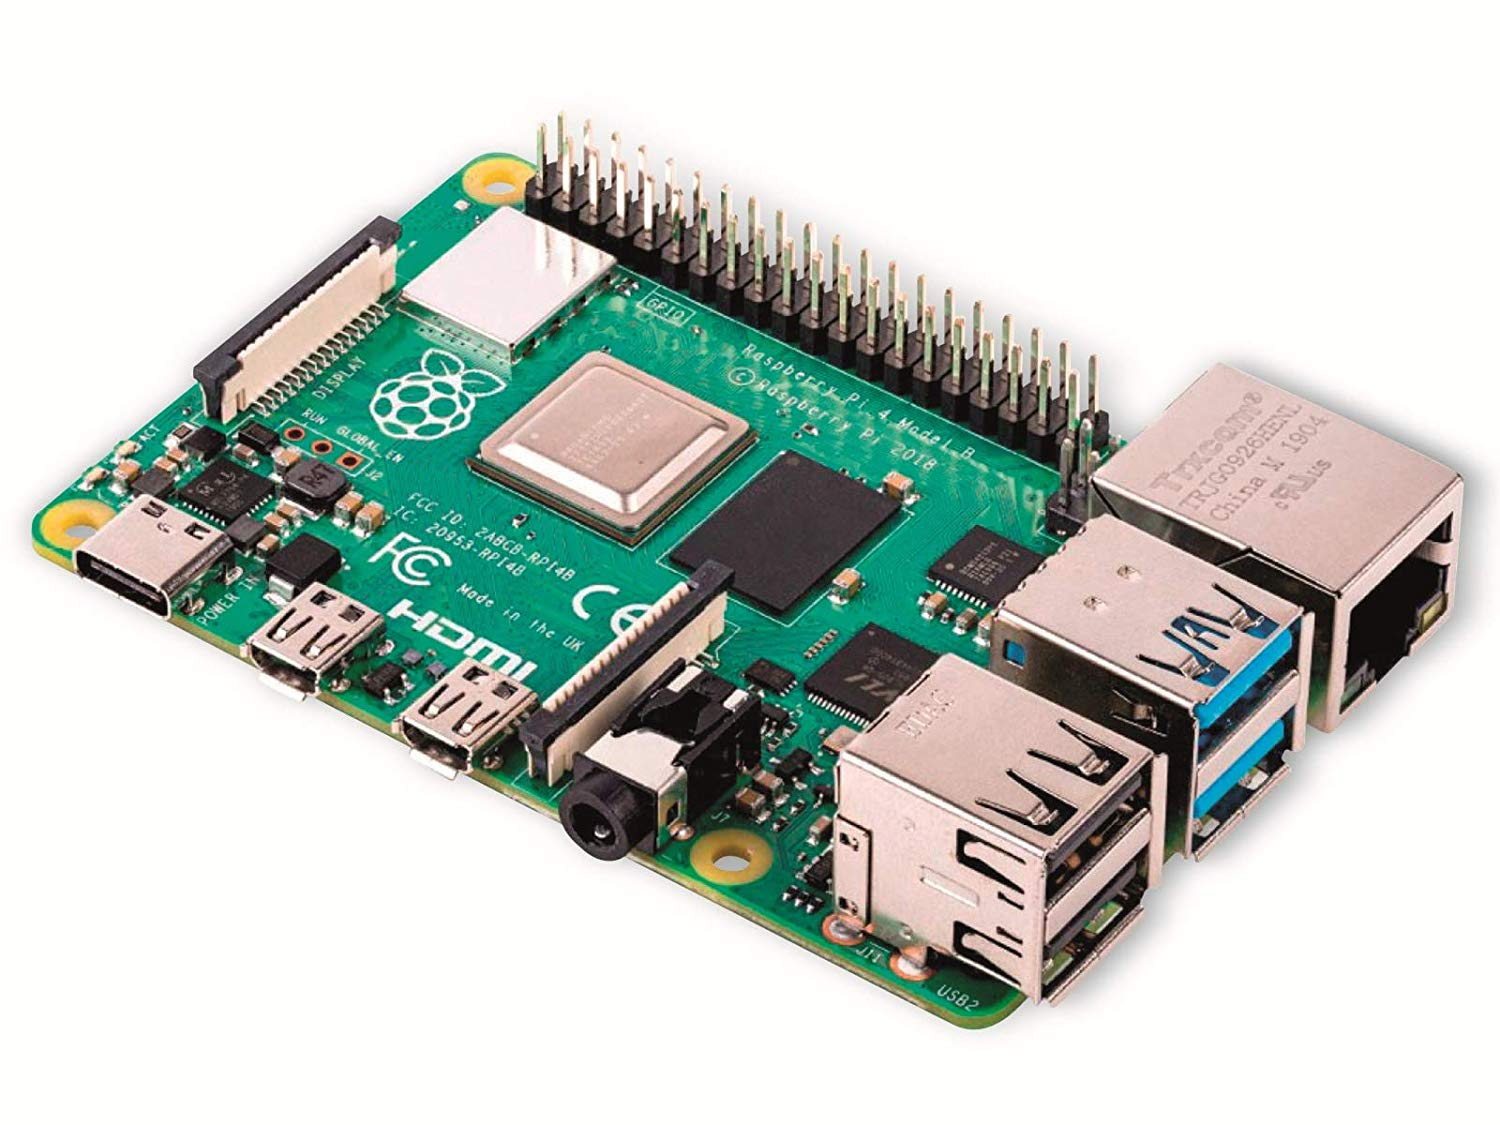
\includegraphics[width=2.5cm]{figure/raspberry 4B.jpg} &
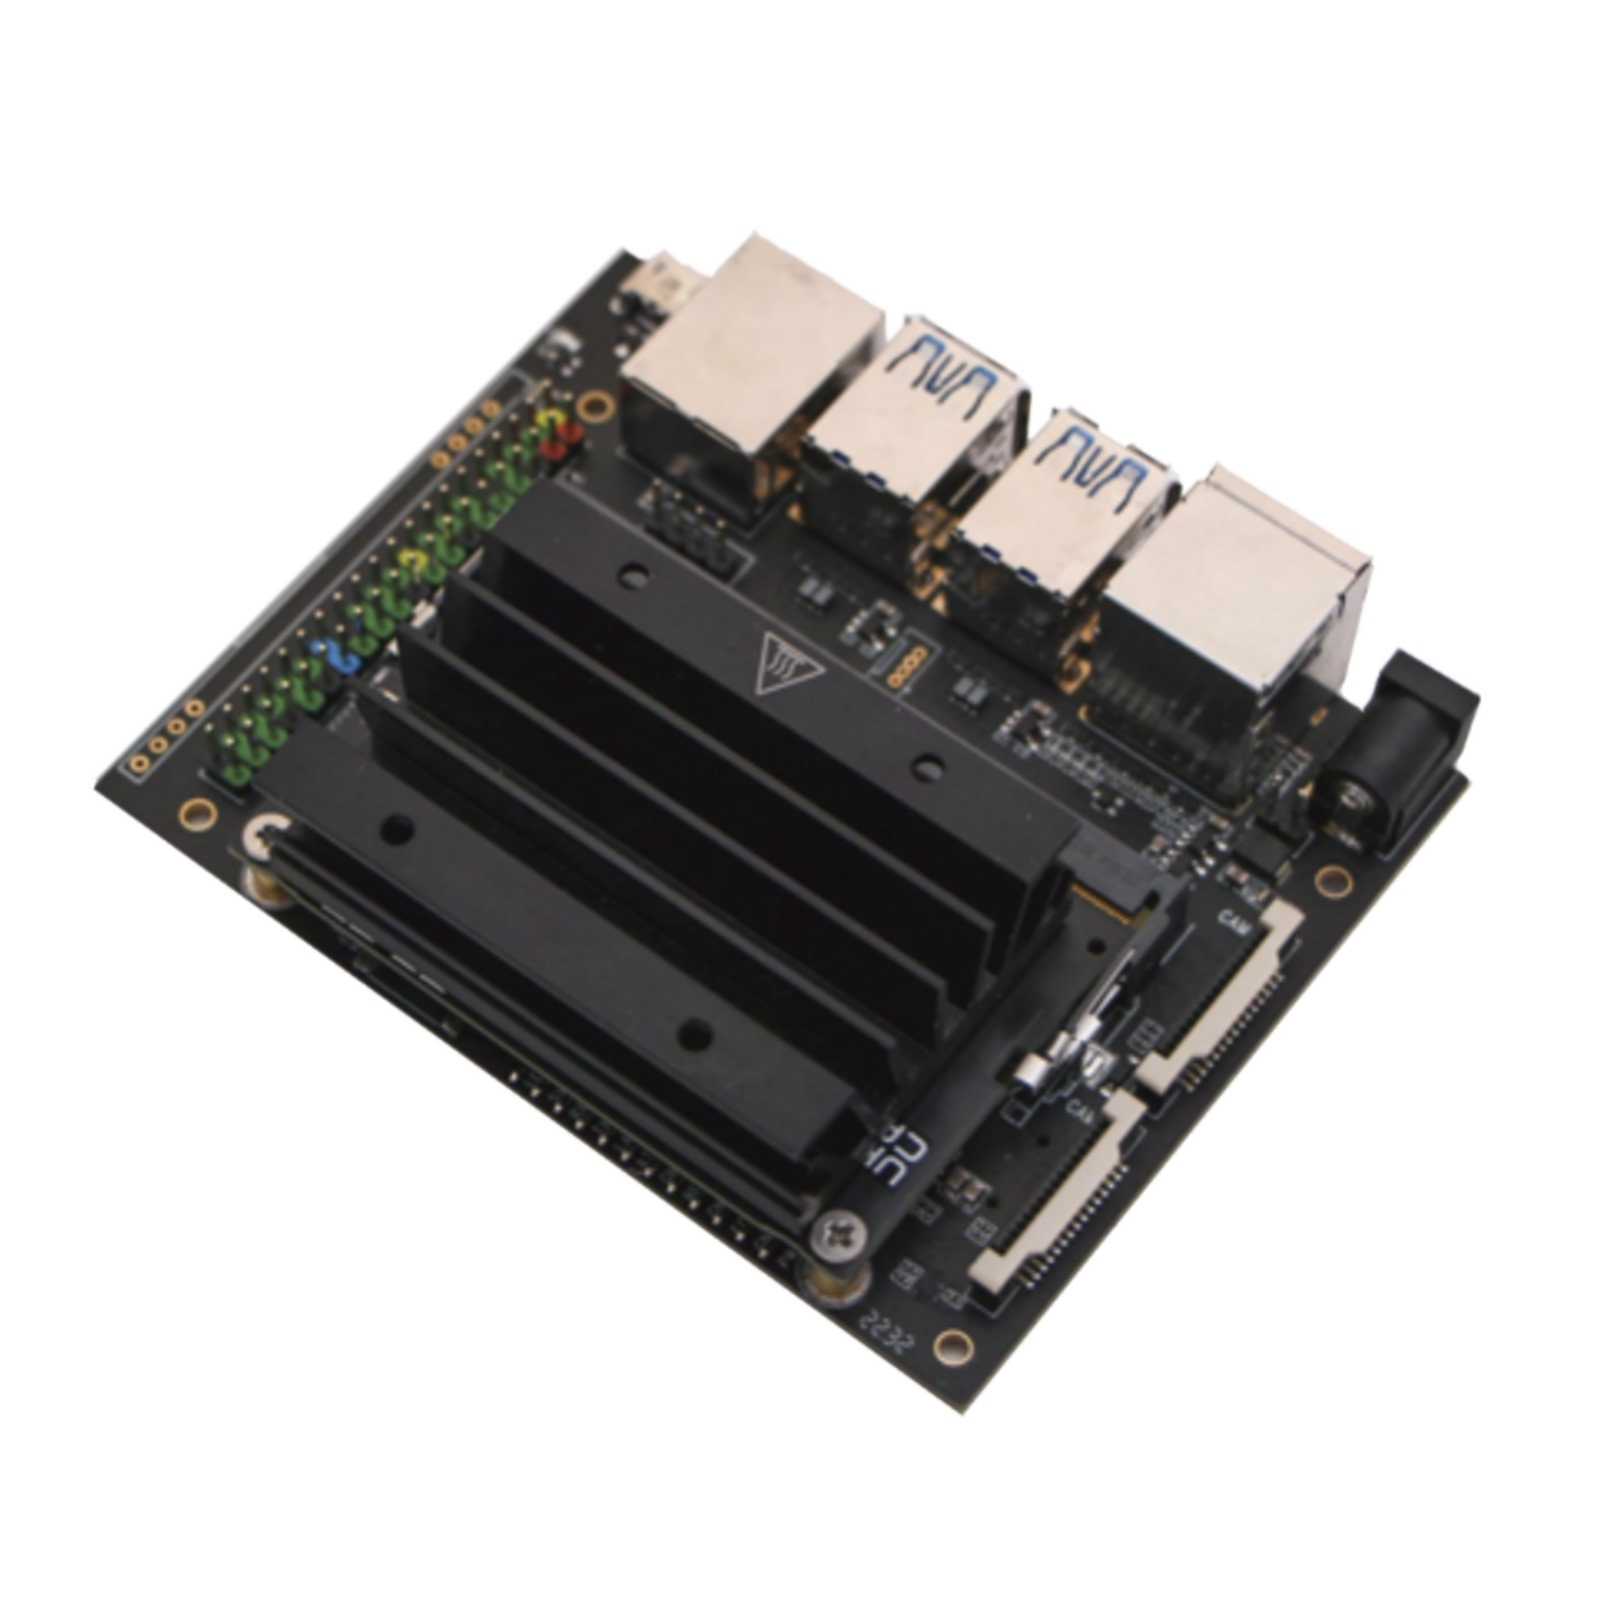
\includegraphics[width=2.5cm]{figure/Nvivid.jpg} \\
\hline

\textbf{RAM} &
2GB / 4GB / 8GB &
4GB \\
\hline

\textbf{Clock Speed} &
1.5GHz &
1.43GHz \\
\hline

\textbf{Connectivity} &
Built-in WiFi / Bluetooth / Ethernet &
Ethernet only \\
\hline

\makecell{\textbf{Dimensions} \\ \textbf{(mm)}} &
85.6 x 56.5 &
100 x 80 \\
\hline

\textbf{GPU} &
Broadcom VideoCore VI &
128-core Maxwell GPU \\
\hline

\textbf{Price} &
Starts from \$60 \cite{amazon_raspberry_pi4_modelb} &
Starts from \$99 \cite{seeedstudio_jetson_nano} \\
\hline

\end{tabular}
\label{tab:single_board_computers}
\end{table}

Raspberry Pi 4B is selected as the main microcontroller of the interactive screen because of the community support it has gathered, multimedia capabilities, and built-in wireless connectivity. Compared to Jetson Nano, it already comes autonomous with WiFi and Bluetooth, thus simplifying communication with the wearable device. The Raspberry Pi 4B also features sufficient processing power and RAM to support real-time video and multimedia content required to calm down the child. Its compact nature, lowered price, and ease to develop render it ideal for use in assistive wearable technology projects like the current one.

\paragraph{Display \\[0.3cm]}
The display function of the interactive screen is among the main parts tasked with displaying comforting images to the child as animation, pictures, or simple games. In addition, when emotionally upset, the child is encouraged to work on the screen directly by means of drawings or scribbles, which may be used as an expressiveness tool to alleviate stress. Hence, display responsiveness and touch are inherent elements.There are two available options for display to choose from shown in Table 3.7.

\clearpage
\renewcommand{\arraystretch}{1.8} % زيادة المسافة بين الصفوف

\begin{table}[h]
\centering
\caption{Differences between standard LCD and TFT LCD.}
\vspace{0.5em}

\begin{tabular}{|>{\centering\arraybackslash}m{4cm}
                |>{\centering\arraybackslash}m{4cm}
                |>{\centering\arraybackslash}m{4cm}|}
\hline
\textbf{Characteristic} &
\textbf{Standard LCD} &
\textbf{TFT LCD} \\
\hline

\textbf{Image} &
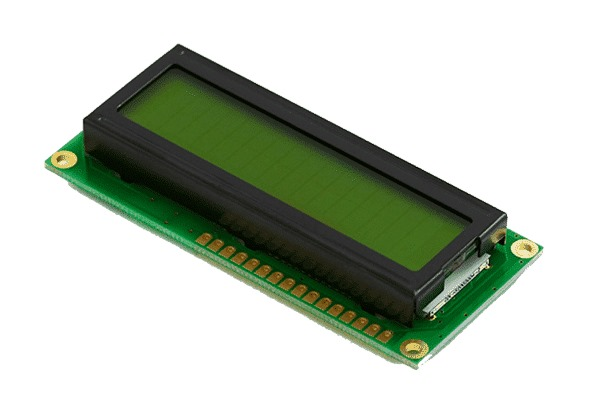
\includegraphics[width=2.5cm]{figure/standardLcd.jpg} &
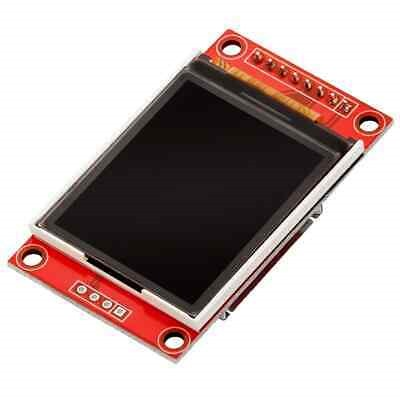
\includegraphics[width=2.5cm]{figure/TFT.jpg} \\
\hline

\textbf{Color Display} &
Typically monochrome or limited color &
Full color \\
\hline

\textbf{Brightness} &
Low to moderate &
High brightness with backlight \\
\hline

\textbf{Viewing Angle} &
Narrow &
Wide viewing angle \\
\hline

\textbf{Refresh Rate} &
Slow (suitable for static images/text) &
Fast (supports animations and videos) \\
\hline

\textbf{Touchscreen Support} &
Rare or not supported &
Widely available with resistive/capacitive options \\
\hline

\textbf{Power Consumption} &
Low &
Moderate \\
\hline

\textbf{Image Quality} &
Basic &
High resolution and sharpness \\
\hline

\textbf{Response Time} &
Slow &
Fast \\
\hline

\textbf{Cost} &
$\approx\$2$ \cite{alibaba_lcd_module_2004} &
$\approx\$7$ \cite{alibaba_lcd_sizes}\\
\hline

\textbf{Interface Options} &
Parallel or serial (limited compatibility) &
SPI, I2C, and parallel (well-supported by ESP32) \\
\hline

\end{tabular}
\label{tab:lcd_display_comparison}
\end{table}

\clearpage
TFT LCD was chosen for the ability to display colorful, reactive images and respond to touch,  which is necessary for soothing and captivating the child.  It can be used for scribbling or drawing when the child is upset, offering a healthy outlet. Unlike standard LCDs, TFT screens provide better brightness, viewing angles, and faster refresh rates, making them ideal for animations and content. Despite slightly higher power use, their benefits in usability and expressiveness make TFT LCD the best fit for this project.


\paragraph{Speaker \\[0.3cm]}
The speaker component is essential in offering auditory feedback to the child during emotional distress. The feedback may be soothing music, calm nature, or simple audio messages. Choosing a speaker that will offer clear, pleasant, and non-intrusive sounds is critical, especially for children with autism, who are sound-sensitive.There are two available options for speakers to choose from shown in Table 3.8. \\[0.1cm]

\renewcommand{\arraystretch}{1.8} % زيادة المسافة بين الصفوف

\begin{table}[h]
\centering
\caption{Differences between USB Speaker and Bluetooth Speaker Module (MH-M28)}
\vspace{0.5em}

\begin{tabular}{|>{\centering\arraybackslash}m{4cm}
                |>{\centering\arraybackslash}m{4cm}
                |>{\centering\arraybackslash}m{4cm}|}
\hline
\textbf{Characteristic} &
\textbf{USB Speaker} &
\textbf{Bluetooth Speaker Module (MH-M28)} \\
\hline

\textbf{Image} &
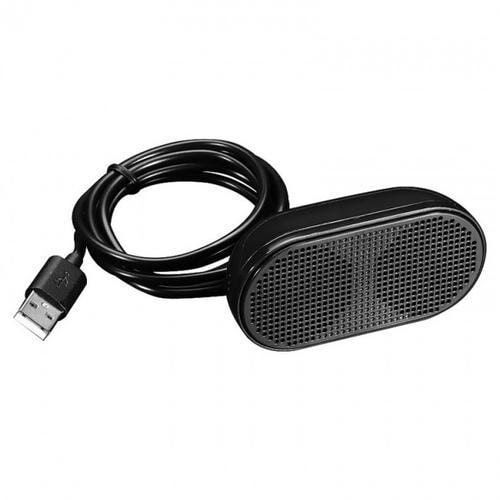
\includegraphics[width=2.5cm]{figure/USB speaker.jpg} &
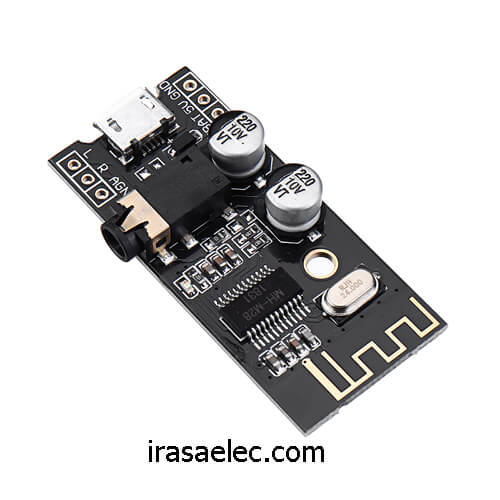
\includegraphics[width=2.5cm]{figure/Blutooth speaker.jpg} \\
\hline

\textbf{Audio Type} &
Digital audio via USB &
Wireless audio via Bluetooth \\
\hline

\textbf{Playback Quality} &
High quality, stable &
High quality, stable sound \\
\hline

\textbf{Integration} &
Requires USB host support &
Easy pairing with phones or microcontrollers \\
\hline

\textbf{Control Method} &
Controlled by USB host (e.g., Raspberry Pi) &
Controlled by paired Bluetooth device \\
\hline

\textbf{Power Consumption} &
Moderate to high &
Moderate \\
\hline

\textbf{Connectivity} &
Wired (USB) &
Wireless (Bluetooth) \\
\hline

\textbf{Price} &
$\approx\$14$ \cite{robotistan_usb_speaker} &
$\approx\$7$ \cite{flipkart_bluetooth_receiver} \\
\hline

\end{tabular}
\label{tab:speaker_comparison}
\end{table}

The USB Speaker was chosen due to its wired connection that is stable, sound output of good quality, and suitability for devices like Raspberry Pi or similar controllers that can be used as a USB host. It can be ideal in offering stable audio feedback with no chance of wireless module pairing issues. It is simple and
rugged, thus ideal for use in children with Autism Spectrum Disorder stress management systems.

\section{Software Components and Design Alternatives}
This part explains the main software components of the Smart Assistant System for Children with Autism, compares possible design choices, and justifies the selected options based on project requirements.
\subsection{Stress Detection}
The stress detection is the system's core, determining if the child is under stress. This detection is essential for alerting specialists and for triggering the feedback mechanisms, be it visual or auditory. The system continuously collects data and analyzes it from the Galvanic Skin Response sensor (GSR), Heart Rate sensor (HR), and Motion sensor sensor, HR sensor, and Motion sensor to classify an emotional state of the child. This detection has to be efficient and reliable in decision making. So, we have listed different options to use as a detector.
\subsubsection{Support Vector Machine (SVM)}
SVMs are a set of supervised learning methods used for classification, regression and outlier detection \cite{scikit_svm}. SVMs are common tools for classification. They find the hyperplane that best separates different classes in a high-dimensional space. By training an SVM model with labeled physiological data, it can learn variations existing between emotional states, thus making the SVM most effective in multi-class classification problems. In our project, SVMs can be used to determine whether physiological response occurs because of stress or due to physical activity, thus providing greater reliability to the stress detection system \cite{mdpi_sensors_wearable}.

\subsubsection{ Random Forest}
Random Forests are groups of decision trees that work together to make a final prediction. Each tree tries to classify independently, with the result finally depending on majority voting between all the trees \cite{pmc_sensors_asd}, as shown in Figure 3.1. The algorithm is implemented in this project for the classification of children's emotional states into "stressed" or "relaxed" using physiological sensor data. Each decision tree looks at only a subset of data and makes a vote toward the final prediction. \\[0.2cm]

\begin{figure}[h]
    \centering
    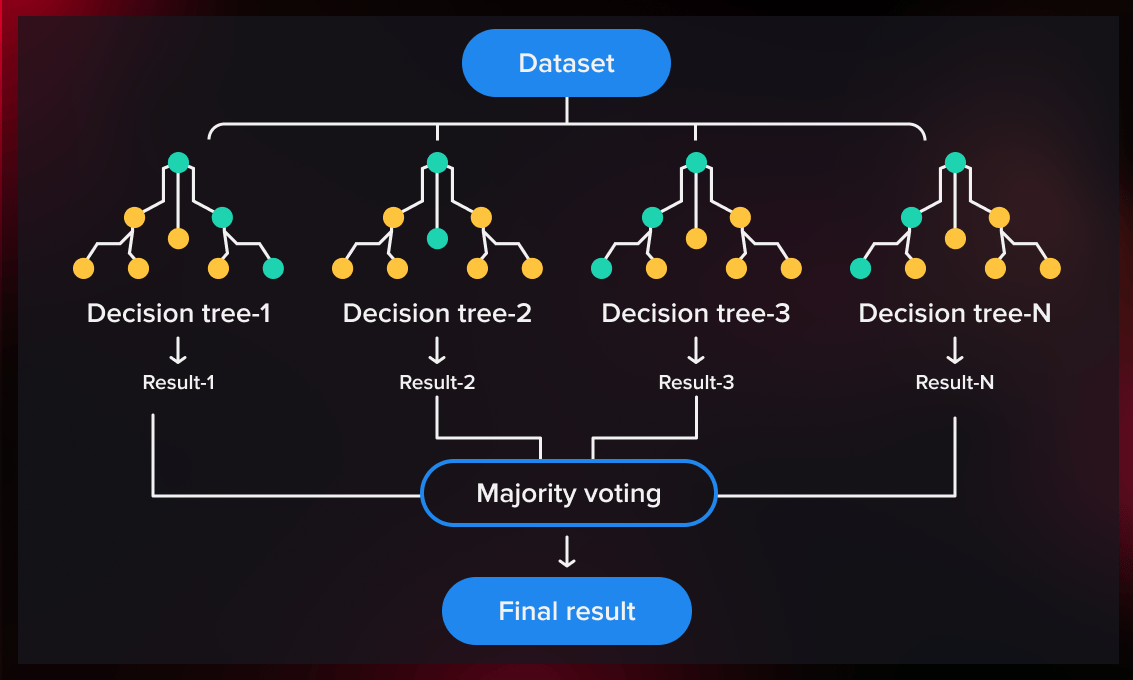
\includegraphics[width=0.5\textwidth]{figure/Random Forest2.png}
    \caption [Random Forest]{Random Forest \cite{serokell_random_forest}}
    \label{fig:system_description}
\end{figure}

Our choice of the algorithm to be used for stress detection is the Random Forest algorithm instead of Support Vector Machine (SVM) because SVM requires extensive parameter tuning and may not scale efficiently with high-dimensional, non-linear physiological data. In contrast, Random Forest being an ensemble method performs better with complex data, is more robust to noise, and requires minimal parameter optimization \cite{geeksforgeeks_rf_vs_svm}.

\subsection{Communication Protocols}
In our project, we define protocols between different system components for communication and data interchange. The protocols allow system integration and operability. The protocols include Wi-Fi that enables a fast wireless network for data transfer, BLE  for short-range wearable communication, and MQTT which is a lightweight messaging protocol for device updates as described in Table 3.9 to help selection based on project needs and limitations. Their particular characteristics are provided to support decisions. \\[0.3cm]
Additionally, since our system includes a mobile app for specialists, the selected protocols must integrate seamlessly with the application development environment. The app will be developed using React Native to support both Android and iOS devices.

\clearpage
\renewcommand{\arraystretch}{1.8} % زيادة المسافة بين الصفوف

\begin{table}[h]
\centering
\caption{ Differences between Communication protocols}
\vspace{0.5em}

\begin{tabular}{|>{\centering\arraybackslash}m{3.5cm}
                |>{\centering\arraybackslash}m{3.5cm}
                |>{\centering\arraybackslash}m{3.5cm}
                |>{\centering\arraybackslash}m{3.5cm}|}
\hline
\textbf{Feature} &
\textbf{BLE \cite{novelbits_ble_power}} &
\textbf{Wi-Fi \cite{techtarget_wifi}} &
\textbf{MQTT \cite{hivemq_mqtt}} \\
\hline

\textbf{Type} &
Short-range Wireless Communication &
High speed Wireless Networking &
Publish-Subscribe Protocol (Application Layer) \\
\hline

\textbf{Use Case} &
Communication between wearable device and mobile app &
Data transfer between mobile app and interactive display &
IoT messaging, notifications, sensor updates \\
\hline

\textbf{Connection Type} &
Intermittent (low duty cycle) &
Persistent (infrastructure or P2P) &
Persistent (broker-based) \\
\hline

\textbf{Reliability} &
Medium (depends on interference and environment) &
High (reliable via TCP/IP) &
High (QoS levels 0, 1, 2) \\
\hline

\textbf{Overhead} &
Low &
High (due to TCP/IP stack) &
Low \\
\hline

\textbf{Power Usage} &
Very low &
High &
Low \\
\hline

\textbf{Range} &
10--100 meters &
Up to 100 meters &
Depends on network (typically local/Wi-Fi coverage) \\
\hline

\textbf{Latency} &
Low &
Moderate &
Very Low (ideal for real-time alerts) \\
\hline

\end{tabular}
\label{tab:ble_wifi_mqtt}
\end{table}


For our project, we choose Wi-Fi and BLE. Short-range communication to mobile apps from wearables is provided by BLE and is ideal for sensors, because of its low power consumption. Wi-Fi connectivity allows for stable and fast data transfer between the interactive display and mobile app. Both options offer a suitable mix of efficiency, performance and connectivity.


\clearpage
\section{Conceptual system description}
The conceptual system design here and the system block diagram in the next figure integrate multiple physiological sensors (Grove galvanic skin response, Heart Rate, Motion) for data collection, a ESP-WROOM- 32 processing unit to detect stress. a LED ring is used as a timer for transition between activities and the specialist can set the time for activity. It will send notifications to a specialist's mobile app when it detects stress. The specialist then uses an interactive screen with audio-visual feedback to provide calming interventions for the child’s sensory sensitivities. \\[0.2cm]

\begin{figure}[h]
    \centering
    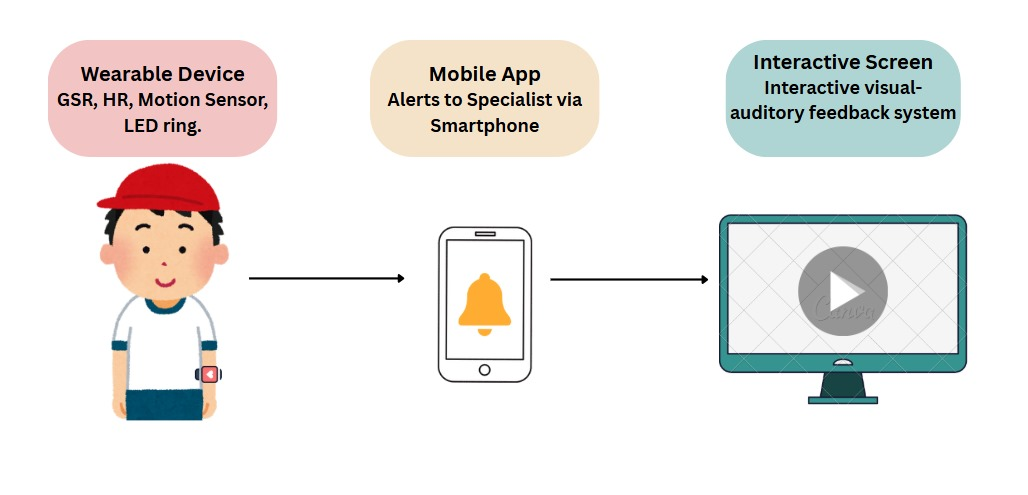
\includegraphics[width=0.7\textwidth]{figure/conceptual diagram2.jpg}
    \caption{ System conceptual diagram } 
    \label{fig:system_description}
\end{figure} 


\begin{figure}[h]
    \centering
    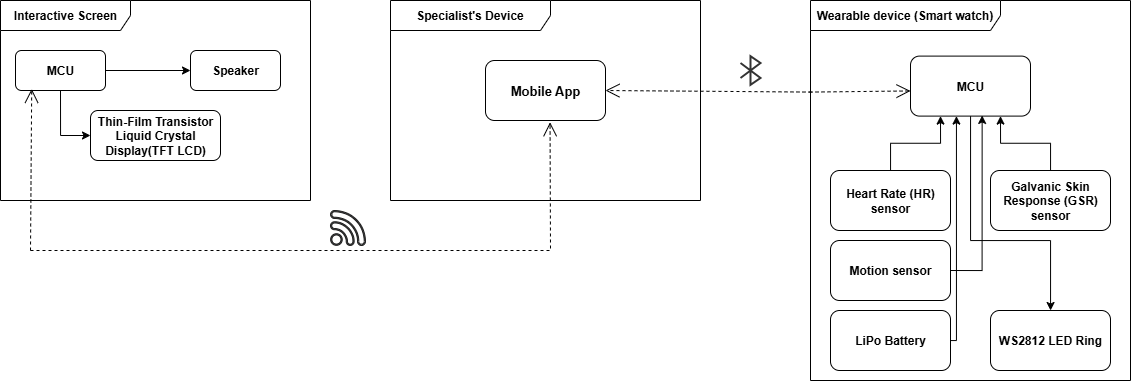
\includegraphics[width=\textwidth]{figure/blockdiagram4.drawio.png}
    \caption{ System block diagram}
    \label{fig:system_description}
\end{figure}

% \clearpage
\section{ Algorithms and Methodologies}
\subsection{Stress Detection Pseudo Code}
This pseudo code defines the detection of stress using physiological sensors,to distinguish between physical exercise and emotional stress, physiological signals Heart Rate (HR) and Galvanic Skin Response (GSR) are processed together with motion sensor signals. Stress is identified only when physiological signals are high with little physical movement. This helps avoid false positives due to exercise or play. 



\begin{tcolorbox}[colback=black!5!white, colframe=black!75!white, title=Pseudo Code for Stress Detection]
\begin{verbatim}
gsr = readGSR()
hr = readHeartRate()
motion = readMotionLevel()
if motion < motion_threshold:
    # Low motion: More likely to be emotional stress
    if gsr > GSR_threshold and hr > HR_threshold:
        stress_level = "High"
    elif gsr > GSR_threshold:
        stress_level = "Medium"
    else:
        stress_level = "Normal"
else:
    features = extractFeatures(gsr, hr, motion)
    stress_level = predictWithRandomForest(features)
\end{verbatim}
\end{tcolorbox}

\subsection{Interactive Screen Control Pseudo Code}
The following pseudo code outlines the core workflow of the Interactive Screen subsystem. After the specialist receives a stress alert via the mobile application, they can directly use the screen’s touch interface to adjust brightness, audio, and visual content, or control from mobile application. \\[0.3cm]

\begin{tcolorbox}[colback=black!5!white, colframe=black!75!white, title=Pseudo Code for Interactive Screen Control]
\begin{verbatim}
event = receive_event()

# Use touch screens to adjust brightness, audio, and visual content 
if event == "TOUCH_INPUT":
    open_control_menu()
    apply_changes_from_touch()

# Manual control command from mobile app
if event == "ADJUST_FEEDBACK":
    set_brightness(value)
    set_audio_volume(value)
    show_animation(content_id)

# Stop all interventions (via touch or app)
if event == "STOP_FEEDBACK":
    stop_audio()
    reset_brightness()
    clear_screen()
\end{verbatim}
\end{tcolorbox}

\clearpage
\subsection{Sequence diagram}

The sequence diagram shows the stress detection system and support task transitions , it shows the flow from detecting the stress signs from the sensors in the wearable device to alerting the specialist to take the suitable decision. \\[0.3cm]


\begin{figure}[h]
    \centering
    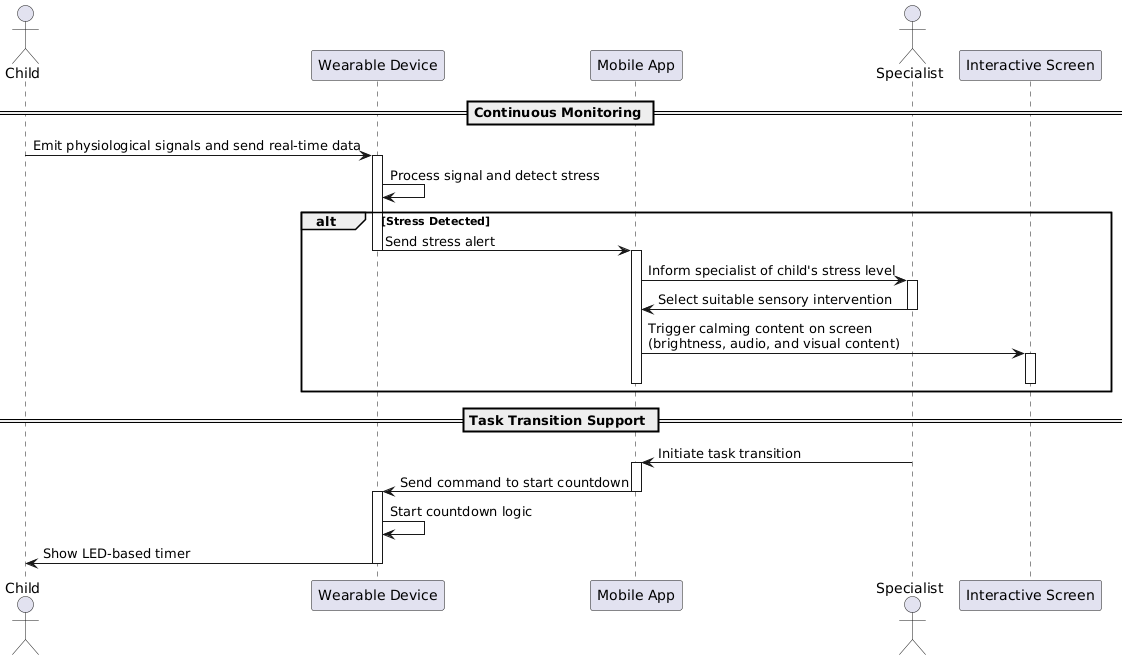
\includegraphics[width=\textwidth,height=0.8\textheight,keepaspectratio]{figure/seq3.png}
    \caption{ Sequence diagram}
    \label{fig:system_description}
\end{figure}


\clearpage
\section{ Schematic diagram}
The schematic diagram shows the hardware layout of the wearable device.The ESP32 microcontroller serves as the central unit, connected to the GSR sensor,MPU6050 motion sensor and the MAX30102 heart rate sensor for collecting physiological data. It also shows the WS2812 LED ring that provides the visual feedback.

\begin{figure}[h]
    \centering
    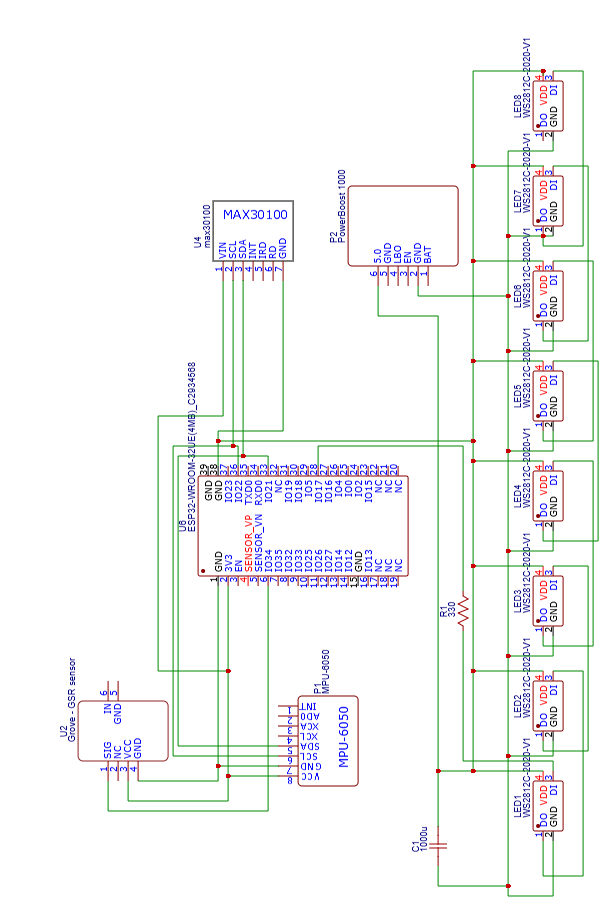
\includegraphics[width=0.7\textwidth,height=0.8\textheight,keepaspectratio]{figure/Schematic_wearable2.png}
    \caption{ Schematic diagram of wearable device}
    \label{fig:system_description}
\end{figure}

\clearpage
The schematic diagram here shows the hardware layout of the interactive screen module. A Raspberry Pi 4B serves as the main processing unit, interfacing with a TFT LCD display through SPI communication for visual output. A USB speaker is connected to provide audio feedback.
\begin{figure}[h]
    \centering
    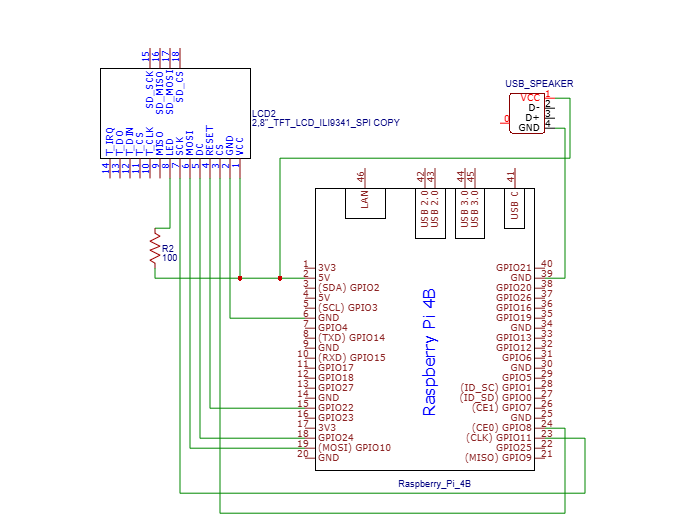
\includegraphics[width=\textwidth,height=0.8\textheight,keepaspectratio]{figure/Schematic_AutismSense_InteractiveScreen2.png}
    \caption{ Schematic diagram of Interactive Screen}
    \label{fig:system_description}
\end{figure}

\section{Summary}
In this chapter, we have discussed the system hardware and software components with their alternatives. The conceptual description of the system and the general flow of the system with all necessary diagrams are presented, too.

\chapter{Conclusion}
\section{Summary}
During this semester, we prepared the Introduction chapter. In Chapter One we wrote the project's background, problem statement, aims, objectives, requirements, system description, and limitations. We also completed Chapter Two, where we provide an overview of definition and classifications for Autism, and sensory processing difficulties in Autistic children and a literature review that compares our project to similar ones. Finally, in Chapter Three we outline the project’s design, encompassing both hardware and software aspects, discuss design choices, the conceptual background of the software, sequence diagram and presents a schematic diagram.

\section{Conclusion}
During this semester, we have completed the analysis and design of the parts of the project as well as designed the entire architecture of the project. The step that was done is the analysis part, where we analyzed some assumptions regarding children with Autism Spectrum Disorder (ASD) in terms of difficulty to emotionally handle and change between one task to another. In addition, based on the analysis, we defined what will be the goals of the proposed system. Moreover, we have designed the entire architecture of the system as well as chosen which hardware and software components will be in the system. We have designed detailed designs of diagrams for the wearable device and the interactive screen.\\[0.1cm]

For next semester, we plan to begin the implementation of the prototype of the system and test and evaluate to confirm the system’s functionality and reliability.

\printbibliography[title={References}, heading=bibintoc]

% أول صفحة مع العنوان + إدراجها في الفهرس
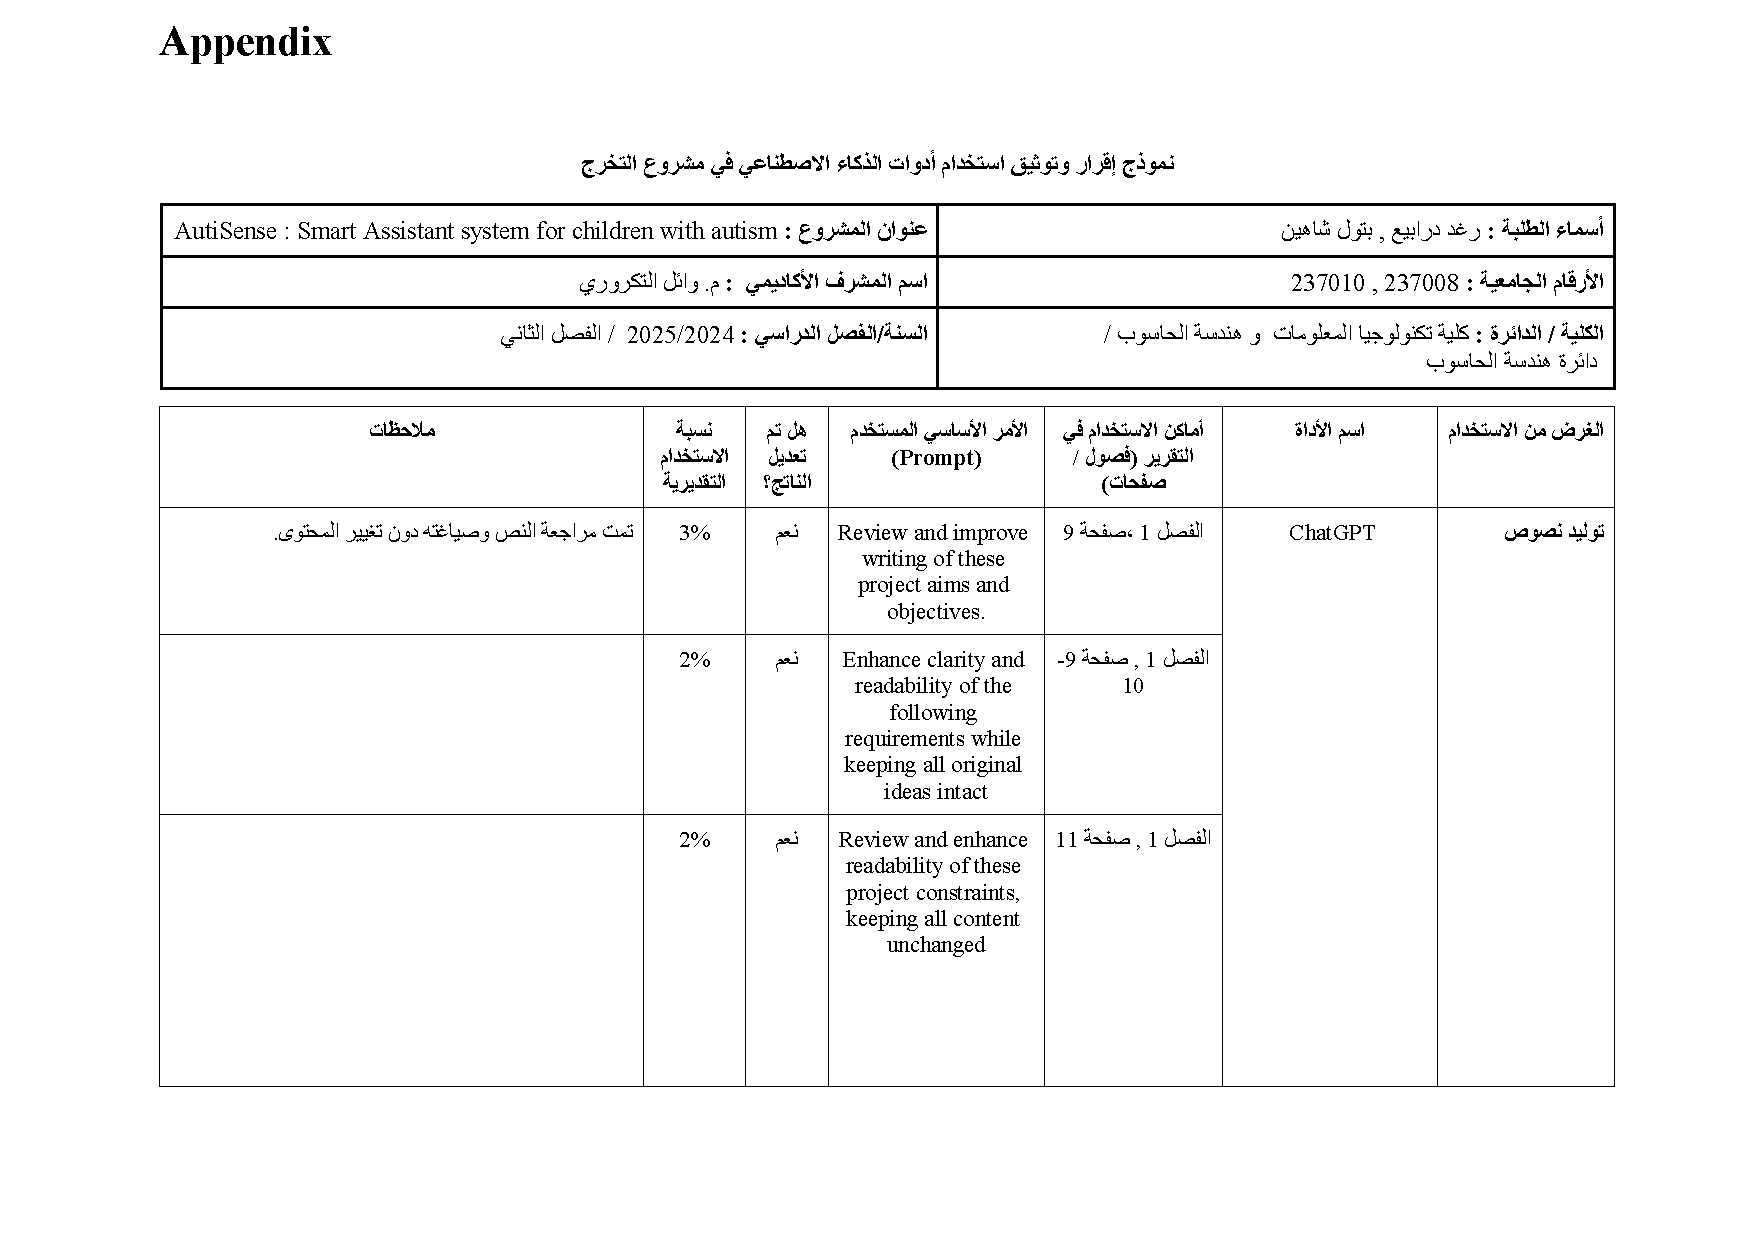
\includepdf[
  pages=1,
  pagecommand={
    \phantomsection
    \addcontentsline{toc}{chapter}{Appendix}
    \thispagestyle{plain}
  }
]{aiedit.pdf}

% باقي الصفحات (2 و 3) بدون عنوان إضافي
\includepdf[
  pages=2-,
  pagecommand={\thispagestyle{plain}} % يضيف ترقيم للصفحات المتبقية
]{aiedit.pdf}

% \printbibliography[title={References}]

% \renewcommand{\bibname}{References} % للكتب والتقارير


% \chapter*{Appendix}
% \begin{figure}[h]
%     \centering
%     \includegraphics[width=0.7\textwidth]{}
% \end{figure}


% دمج صفحة PDF كجدول تحت النص
% \begin{tikzpicture}[remember picture,overlay]
% \node[anchor=north,yshift=-2cm] at (current page.north) {%
%     \includegraphics[page=1, width=\textwidth]{AI-Usage.pdf}%
% };
% \end{tikzpicture}

% % ترقيم الصفحة
% \thispagestyle{plain}

% Appendix
% \includepdf[pages=-, pagecommand={\thispagestyle{plain}}]{AI-Usage.pdf}

% \chapter*{Appendix}
% \addcontentsline{toc}{chapter}{Appendix}
% \begin{tikzpicture}[remember picture,overlay]
% \node[anchor=north] at (current page.north) {
%     \includegraphics[page=1, width=\textwidth]{AI-Usage.pdf}
% };
% \end{tikzpicture}

% % ترقيم الصفحة
% \thispagestyle{plain}



\end{document}
